\documentclass[english]{report}
\frenchspacing

\usepackage[marginparwidth=2.9cm, marginparsep=.1cm]{geometry}
\geometry{a4paper}

\usepackage[shadow,color=green!20,textsize=tiny,disable]{todonotes}
\def\tod#1{\todo{\sf #1}}
\def\todr#1{\todo[backgroundcolor=red!10, linecolor=red]{\sf #1}}

\usepackage{titlepic}

\usepackage{natbib}
\usepackage{topcapt}
\usepackage{fancyvrb}
\usepackage{relsize}
\usepackage{graphicx}
\usepackage{amssymb,amsmath}
\usepackage{color}
\usepackage{hyperref}

\def\sep{\hbox{-}}
\def\int{\hbox{\texttt{\~}}}
\def\tbf#1{\textbf{#1}}
\def\tcb#1{\textcolor{blue}{\ttt{#1}}}
\def\ttt#1{\texttt{#1}}
\def\var#1{\textquotesingle #1\textquotesingle}


\DefineVerbatimEnvironment{kappasource}{Verbatim}{baselinestretch=1,fontsize=\relsize{-1},commandchars=\\\{\}}
\DefineVerbatimEnvironment{bnfsource}{Verbatim}{baselinestretch=1,fontsize=\relsize{-1},commandchars=\\\{\}}
\DefineVerbatimEnvironment{pseudocode}{Verbatim}{baselinestretch=1,fontsize=\relsize{-1}}

\hypersetup{colorlinks=true,citecolor=blue,linkcolor=blue,urlcolor=blue}

\newcommand{\newbnf}[1]{\colorbox[rgb]{0.8,0.8,1}{#1}}

\title{Spatial Kappa Simulator\thanks{The simulator is available from GitHub as the source Eclipse project, or as a single executable jar file. Both can be found at \url{https://github.com/lptolik/SpatialKappa/}. 
}\\User Guide\\v2.1.1}
\author{
Anatoly Sorokin\thanks{The University of Edinburgh, School of Informatics, Edinburgh, UK} 
\and Oksana Sorokina\footnotemark[2]
\and 
Donal Stewart\thanks{DemonSoft.org, UK}
}
\titlepic{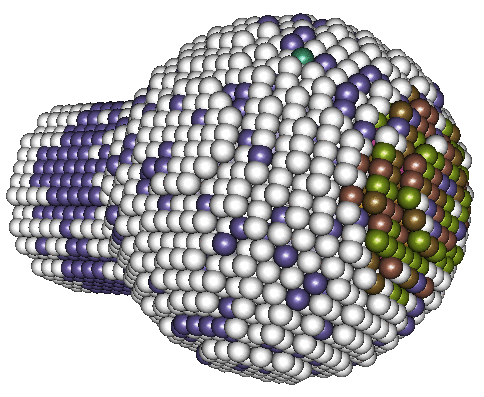
\includegraphics[width=250pt]{images/spine-cover} }

\begin{document}

\maketitle


\section*{Acknowledgements}
The development of Spatial Kappa was funded in part by the Edinburgh Centre for Synthetic and Systems Biology (SynthSys). SynthSys was funded as a Centre for Integrative Systems Biology (CISB) jointly funded by BBSRC and EPSRC (reference \href{http://www.research.ed.ac.uk/portal/en/projects/centre-for-systems-biology-at-edinburgh-bbd0196211(66deffd6-c28b-44d7-adaf-9b574307c62b).html}{BB/D019621/1}) for the period 2007--2012.

\tableofcontents

%\chapter{Kappa Language Extensions}

Note on terminology. In the following 'cell' can mean either a living cell, or a cell within a defined compartment. Hopefully the meaning in each situation will be clear from the context. Current Kappa rules are referred to as 'transform' rules as they cause some form of transformation of their substrates, be it change of agent state, agent creation or deletion, agent binding or unbinding. Species is mostly used to refer to a particular agent or complex in the model.

Also this document uses the terms 'language' and 'calculus' interchangeably, for example $\kappa$-calculus and Kappa language. Generally the term calculus is used when referring to the formal definition, and language where referring to models defined in Kappa, as they are represented in the Kappa language syntax.

\section{Existing Kappa language}

The current Kappa language consists of the following constructs, as described in the Simplx documentation \citep{krivine2009}. A more formal description of the language grammar (including the spatial extensions) is given in appendix \ref{chap:spatialGrammar}.

\textbf{Comments}:

\begin{kappasource}
# This is a comment
\end{kappasource} 

\textbf{Agents}:

\begin{kappasource}
AgentName()
AgentName(stateWithValue~stateValue, stateWithNoValue, unboundSite, boundSite!1)
\end{kappasource} 


\textbf{Transform rules}:

\begin{kappasource}
'state change' A(state~old) -> A(state~new) @ 0.1
'binding'      A(bindsite),B(bindsite) -> A(bindsite!1),B(bindsite!1) @ 0.1
'unbinding'    A(bindsite!1),B(bindsite!1) -> A(bindsite),B(bindsite) @ 0.1
'creation'     -> A() @ 0.1
'degradation'  A() -> @ 0.1
'reversible reaction'  A(state~old) <-> A(state~new) @ 0.1,0.2
A(state~old) -> A(state~new) @ 0.1 # Unnamed transform rule
\end{kappasource} 

\textbf{Initial species values}:

\begin{kappasource}
\%init 1000 * (A(state~old),C())            # 1000 of each of A(..) and C()
\%init 2000 * (A(bindsite!1),B(bindsite!1)) # 2000 of the bound complex A(..),B(..)
\end{kappasource} 

\textbf{Observables and named variables}: Variables can be referenced in perturbation calculations, but do not show in outputs as observations.

\begin{kappasource}
\%obs 'Label' A()  # All agents A()
\%obs A()          # Unnamed observation, will default to 'A()' in outputs
\%obs A(state~old) # All agents matching A(state~old)
\%obs 'binding'    # Activity of the transform rule named 'binding'

\%var 'Named variable' B()
\end{kappasource} 

\textbf{Perturbations}: These only fire a single time, after which they are disregarded for the rest of a simulation.

\begin{kappasource}
# When simulation time exceeds 5 seconds, change the rate of transform rule
#   named 'unbinding' to 10.0
\%mod: \$T > 5 do ’unbinding’:= 10.0

# When the species value mapped to observable 'mRNA' drops below 50
#   set the rate of transform named 'transcribe' to 0.5
\%mod: 'mRNA' < 50 do 'transcribe' := 0.5
\end{kappasource} 

\textbf{Currently unused}: There are some Kappa syntax elements not directly relevant to the spatial extensions, and will not appear in the extended grammar. One is a representation of causal flows, which uses the keyword \verb|%causal|.

\begin{kappasource}
\%causal: ’C@s2’ 
\%causal: {’A..B’,’C@s1’} => ’C@s2’ 
\end{kappasource} 


\section{Concepts to encapsulate}

The spatial Kappa language requires some encoding of the following concepts to be useful.

\begin{itemize}
 \item A description of \textbf{compartments} and their \textbf{dimensions}. A model may have multiple compartments each containing reacting species. The dimensions are necessary to define the shape of a compartment, be it a single cell, a 1 dimensional linear array of cells, a 2 dimensional grid of some form, or a 3 dimensional lattice structure. Relative differences in size of different compartments can be specified, e.g. the reacting volume of a nucleus relative to the surrounding cytosol. Relative differences in shape can also be specified, for example the thin layer of cytosol next to the inner surface of the plasma membrane versus the rest of the cytosol.

 \item A description of \textbf{linkage}, both intra-compartment and inter-compartment. The intra-compartment linkage specification should be rich enough to allow description of multiple structures, e.g. in 1D linear arrays or circles, in 2D square or hexagonal meshes, cylinders or tori, in 3D cubes, filled cylinders, spheres, etc.

 \item A means of \textbf{locating species} within compartments, e.g. all DNA would reside within the nucleus, or cell receptors would be limited to the plasma membrane.

 \item A means of \textbf{locating transform rules} within compartments, e.g. DNA transcription is isolated to the nucleus. The language should also allow the same transform rule to be specified with different rates depending on the location of the reacting species.

 \item A description of the \textbf{transport} (active or diffusive) of species within a compartment or between compartments along previously described linkage structures. The rates of transport should be general to all species, or species specific.

\end{itemize}


\textbf{Additional concepts}

\begin{itemize}
 \item \textbf{Granularity} within compartments. It would be useful to be able to specify locations at the level of compartments or single cells within a compartment. This would allow the model to represent, for example, a signal cascade being initiated as one point in the cytosol, and the resulting signal molecules being diffused through the cytosol. 

 \item \textbf{Backwards compatibility} with basic Kappa. Given the quantity of existing models, the extended language should allow the existing models to work as before without modification. The user should have the choice of not using the spatial aspects of the extended language with no rework penalty.

\end{itemize}


\section{New language constructs}

A full BNF description of the extended Kappa grammar is given in appendix \ref{chap:spatialGrammar}.

\subsection{Compartments and cells}

Compartments are defined as single cells or regular multidimensional arrays of cells as follows
\begin{bnfsource}
'\%compartment:' LABEL ('[' INT ']')*
\end{bnfsource}
For example
\begin{kappasource}
\%compartment: 'Single cell' 
\%compartment: '1d array' [10]       # 10 cells in size 
\%compartment: '2d array' [10][5]    # 10x5 cells in size 
\%compartment: '3d array' [10][5][4] # 10x5x4 cells in size 
\end{kappasource}

Compartments or individual cells within a compartment can be referenced using the following syntax
\begin{bnfsource}
LABEL ( '[' mathExpr ']' )*
\end{bnfsource}
where
\begin{bnfsource}
mathExpr :
  mathAtom OPERATOR mathAtom
  | mathAtom
  
mathAtom :
  '(' mathExpr ')'
  | INT
  | VARIABLE_NAME
  
OPERATOR :
  '+' | '-' | '*' | '/' | '\%'
\end{bnfsource}
For example
\begin{kappasource}
'my compartment'                     # the compartment as a whole
'my compartment' [0][0][0]           # the first cell in a 3d array compartment
'my compartment' [4]                 # the fifth cell in a 1d linear arrays

'my compartment' [x][y][z]           # variable name usage described in
'my compartment' [x*2][y-1][z+(x*3)] #   compartment links section below
\end{kappasource}

In all situations where compartment references are used, it is only legal to refer to the compartment as a whole by omitting the cell indices, or refer to a single cell, by fully defining the correct number of cell indices to match the dimensions of the compartment. Also, variable names are only permitted in compartment references within compartment link definitions, described below.

\subsection{Compartment links}

The structure of a compartment is further defined by how cells within the compartment are linked to each other and to connected compartments. This linkage is defined as follows
\begin{bnfsource}
'\%link:' LABEL compartmentReferenceExpr ('<->' | '<-' | '->') compartmentReferenceExpr
\end{bnfsource}
Where \verb|compartmentReferenceExpr| is as described above. For example
\begin{kappasource}
\%compartment: '2d array' [10][200]    # 10x200 cells in size 

# Link all cells to their horizontally adjacent neighbours
\%link: 'meshlinks' '2d array'[x][y] <-> '2d array'[x+1][y]

# Link all cells to their vertically adjacent neighbours
\%link: 'meshlinks' '2d array'[x][y] <-> '2d array'[x][y+1]

# Wrap around the cells on the left and right edges to create a cylinder
\%link: 'meshlinks' '2d array'[0][y] <-> '2d array'[9][y]

# Wrap around the cells on the top and bottom edges to create a torus
\%link: 'meshlinks' '2d array'[x][0] <-> '2d array'[x][199]
\end{kappasource}

The above code defines a thin torus composed of a 2d mesh.

Compartment references on the left hand side of the link definitions above may contain either constant values or single variable names, not complex expressions. The variable names are used to define the dimensions which will be iterated through to produce links. Compartment references on the right hand side allow constant values or complex expressions involving the variables defined on the left had side of the expression. It is invalid for the right hand expression to use variables not defined on the left. If setting the values of variables references valid cells on both the left and right, then those cells are deemed to be linked. References which refer to cells outside the dimensions of the compartment are ignored, and no link is created. The references in a link expression can refer to the same compartment, or two different compartments. The modulus operator \verb|%| is useful in defining regular, repeating linkage patterns within the compartment, for example the 2D hexagonal mesh described in appendix \ref{sec:spatialPatterns}.

Multiple link definitions can use the same label (like \verb|meshlinks| in the example above), in which case references to that label elsewhere in the model acts on the union of all the link definitions. This allows complex linkage definitions, for example compartments constructed in the form of a circle or sphere, to be referenced concisely in transport rules.

Further examples of compartment and link specifications for common structures are given in appendix
 \ref{sec:spatialPatterns}.

\subsection{Transport rules}

These rules define the rate at which species move from one compartment (or cell) to another.
\begin{bnfsource}
'\%transport:' (transportName=LABEL)? linkName=LABEL (agentGroup)? transportKineticExpr
\end{bnfsource}
  where
\begin{bnfsource}
agentGroup :
  agent (',' agent)*

transportKineticExpr :
  '@' a=rateValueExpr

rateValueExpr :
  number | '\$INF'   # \$INF means infinite rate
\end{bnfsource}

See appendix \ref{chap:spatialGrammar} for the definition of the remaining constructs. For examples of usage

\begin{kappasource}
# All species diffusing around the torus defined above
\%transport: 'general diffusion' 'meshlinks' @ 0.1

# Immediate exit of the named species through a uni-directional channel.
# Note the label for the transport is optional.
\%transport: 'Ca channel' Calcium() @ \$INF
\end{kappasource}

When referencing bidirectional compartment links (i.e. ones specified with '\verb|<->|', the rate applies equally in either direction across the link. In the second example above, care would need to be taken in defining the compartment link \verb|Ca channel| in the correct orientation.

\section{Additions to existing language constructs}

New clauses were added to existing Kappa language constructs to allow the use of compartments and links. In all cases, existing Kappa syntax is still valid. Where necessary, the optional label in existing Kappa statements is non-optional in statements using compartments to avoid ambiguity. When basic Kappa syntax is used in the context of a spatially aware model, the statement is generally taken to apply to all compartments in the model equally.

\subsection{Transform rules}

The following transform statement was added

\begin{bnfsource}
transformName=LABEL locationExpr transformExpr transformKineticExpr 
\end{bnfsource}
  where
\begin{bnfsource}
transformExpr :
  (a=agentGroup)? ( '->' | '<->' ) (b=agentGroup)?

transformKineticExpr :
  '@' a=rateValueExpr (',' b=rateValueExpr)?
\end{bnfsource}
For example
\begin{kappasource}
# mRNA degradation happens outside the nuclear membrane
'degradation' 'cytosol' mRNA() -> @ 6.21

# Heating of the agent occurs in cell 0 of the cytosol compartment
'heating' 'cytosol'[0] A(state~blue) -> A(state~red) @ 1.0
\end{kappasource}

As mentioned before valid locations are either entire compartments or single compartment cells.

\subsection{Initial values}

The following initial value statement was added

\begin{bnfsource}
initExpr :
  '\%init:' locationExpr INT '*' '(' agentGroup ')'
\end{bnfsource}
For example
\begin{kappasource}
# Distribute 2000 blue agents within the cells of cytosol equally
\%init: 'cytosol' 2000 * (A(state~blue)) 

# Add 500 red agents to cell 5 of the cytosol compartment
\%init: 'cytosol'[5] 500 * (A(state~red)) 
\end{kappasource}

\subsection{Observations}

The following observation statement was added

\begin{bnfsource}
obsExpr :
  '\%obs:' LABEL locationExpr agentGroup
\end{bnfsource}
For example
\begin{kappasource}
# Count all blue agents in all cells of the cytosol
\%obs: 'cytosol blue' 'cytosol' A(state~blue)

# Count all red agents in cell 0 of the cytosol compartment
\%obs: 'red[0]' 'cytosol'[0] A(state~red) 
\end{kappasource}


\bigskip For example models demonstrating the use of the language extensions, refer to appendix \ref{chap:resources}.

\newpage



\section*{What is rule-based modeling?}
Rule-based modeling uses rules to construct models of systems of interacting bio-molecules. The approach  is especially effective for systems with combinatorial complexity, where relatively concise rule-sets may approximate information about a complex biochemical network with enough precision. Proteins that participate in signaling cascades are commonly composed of multiple subunits and binding domains. These domains can mediate more than one domain-domain interaction, and/or allow for the formation or repeated polymeric motifs,
which results in many possible protein complexes. Domain-domain interactions, in turn, are governed by post-translational modifications that provide an additional level of variety. Therefore, when conventional modelling, such as ODEs, takes these elements of molecular structure into account - model sizes grow exponentially (or worse) with the number of interactions.
Instead, graphs can be used to conveniently represent structured objects (such as molecules with there sites and states) and graph-rewriting rules can approximate their interactions. 
A graph-rewriting rule specifies an edge addition or removal when proteins are binding or unbinding. It can also change the state (label) of any component to represent post-translational modification. Each rule accounts for the class of reactions that chemicals with common structure could share. Only information that is important for a particular interaction is taken into account, so that the states and domains that are not involved are ignored. All the reactions that are implied by one rule will be parameterized by the same rate constant, which gives a significant reduction of the model complexity.

\section*{What is Kappa?}
Kappa is a member of the rule-based language family. Its main simulator is KaSim~\citep{KaSimManual2012} now in version 3. To know how plain Kappa is used in a modeling context, the following short note is a good start~\citep{sos08}. A longer article is also available~\citep{concur07}; see also this tutorial~\citep{cav09}.


\section*{What is this User Guide about?}
This manual documents an extension of the Kappa language, called \emph{Spatial Kappa}. Differently from Kappa which assumes that all agents in a model co-exist in an homogeneous and well-stirred volume, in Spatial Kappa, one can define compartments and rules for diffusion within and transport across them. 

The spatial Kappa language %requires some encoding of the following concepts to be useful.
is backward compatible with basic Kappa. Potential users, already familiar with Kappa, should find the extension intuitive.

%Given the quantity of existing models, the extended language should allow 
Existing Kappa models can be run without modifications
---provided they do not incorporate directives related to causality analysis and causal flows.
This allows one to develop a model in a space-less manner first, and to then introduce spatial aspects gradually.

\chapter{Kappa Language Extensions}
Note on terminology: in the following `voxel' means a subunit of a defined compartment;
`species' is used to refer either to a particular agent, or a partial complex of agents, or a full complex ---when we need to be more explicit, we say agent, partial complex, or full complex; usual Kappa rules
are sometimes called transform rules, as they entail the modification of their targets, to stress the difference with transport or diffusion rules which merely displace their targets.


\section{Existing Kappa language}

We start with a brief description of the current Kappa language as defined in the KaSim Reference Manual~\citep{KaSimManual2012}. A formal description of the language including spatial extensions is given in Appendix \ref{chap:spatialGrammar}.

Basic elements in a model can be declared either as agents or tokens. \emph{Agents} are used to represent complex objects with multiple binding sites that can bind/unbind and modify others. They have a discrete number of instances. \emph{Tokens} correspond to simple unstructured objects. They cannot bind to other tokens and agents, and can only appear and disappear. They have continuous concentrations. An agent declaration contains its \emph{signature}, that is to say the information about the agent that will be used in the model, such as its name, its interactions sites and their states. 
%
For instance, the line:
\begin{kappasource}
\%agent: A (x,y~u~p,z~0~1~2) 
\end{kappasource}
declares an agent \Verb+A+ with three binding sites \Verb+x+, \Verb+y+ and \Verb+z+, where \Verb+y+ can exist in two states (\Verb+u+ and \Verb+p+, typically for phosphorylated and unphosphorylated) and \Verb+z+ - in three states, \Verb+0+, \Verb+1+, and \Verb+2+. It is possible to declare an agent with any number of sites, including no sites %(see first line above), 
at all (in which case the agent essentially a token).


%More generally, an agent declaration follows the following syntax:
%
%%\tbf{Agents}:
%
%\begin{kappasource}
%AgentName()
%AgentName(stateWithValue~stateValue, stateWithNoValue, unboundSite, boundSite!1)
%\end{kappasource} 
%

Declared agents are used in turn to define rules which describe their dynamics. A typical rule starts with a name (a string) and contains a left hand side and a right hand side expression together with a corresponding kinetic rate. 
%
%\tbf{Rules}:
%
\begin{kappasource}
'my rule' kappa_expression -> kappa_expression @ rate
\end{kappasource}

Rules can also be bi-directional, in which case one must provide two kinetic rates:
\begin{kappasource}
'my bidirectional rule' kappa_expression <-> kappa_expression @ rate_left_to_right, rate_right_to_left
\end{kappasource}

Rates can be (positive) real numbers as well as algebraic expressions.
Here are examples of the most common types of rules:
%
%\tbf{Transform rules}:
%
\begin{kappasource}
'state change' A(state~old) -> A(state~new) @ 0.1
'binding'      A(bindsite),B(bindsite) -> A(bindsite!1),B(bindsite!1) @ 0.1
'unbinding'    A(bindsite!1),B(bindsite!1) -> A(bindsite),B(bindsite) @ 0.1
'creation'     -> A() @ 0.1
'degradation'  A() -> @ 0.1
\end{kappasource} 

The initial string, i.e. the name of the rule, is optional:
\begin{kappasource}
A(state~old) -> A(state~new) @ 0.1 # Unnamed rule
\end{kappasource} 
(Note above the use of a comment with comment character \Verb+#+.)

Initial conditions are defined in the form of algebraic expressions to be evaluated 
before the initialization of the simulation:
%
%\tbf{Initial conditions}:
%
\begin{kappasource}
\%init 1000 A(state~old),C()            # 1000 of each of A(..) and C()
\%init 2000 A(bindsite!1),B(bindsite!1) # 2000 of the dimer A(..),B(..)
\%var  'n' 100
\%init 'n' (A(),A(y~p)) # 100 instances of A default state A (x,y~u,z~0) and 100 A(x,y~p,z~0) 
\end{kappasource} 
%
%\tbf{Observables and named variables}: 
%

The above snippet of code introduces a \emph{variable} \Verb+'n'+. Once declared, a variable can be referenced in rates, observables, as well as in perturbations (see below). \emph{Observables} define the outputs of the simulation.

\begin{kappasource}
\%obs 'Label' A()  # All agents A()
\%obs A()          # Unnamed observation, will default to 'A()' in outputs
\%obs A(state~old) # All agents matching A(state~old)
\%obs 'binding'    # Activity of the transform rule named 'binding'

\%var 'Named variable' B()
\end{kappasource} 

Variables can be used to trigger specific events named \emph{perturbations} during 
the simulation.
\begin{kappasource}
# When observable 'mRNA' drops below 50 set the rate of 'transcribe' to 0.5
\%mod: 'mRNA' < 50 do 'transcribe' := 0.5
\end{kappasource} 
Perturbations can also condition events on the global time of the simulation:
%
%\tbf{Perturbations}: 
%
\begin{kappasource}
# At time 5, change the rate of 'unbinding' to 10.0
\%mod: [T] > 5 do 'unbinding':= 10.0
\end{kappasource} 

%One is a representation of causal flows, which uses the keyword \Verb+%causal+.
%
%\begin{kappasource}
%\%causal: ’C@s2’ 
%\%causal: {’A..B’,’C@s1’} => ’C@s2’ 
%\end{kappasource} 

\section{New Concepts}


Spatial Kappa introduces a number of new features: compartments, voxels, and channels which are used to defined transport between voxels and compartments, as well as new kinds of `transport' rules which exploit these additional features. We go briefly over an informal presentation of these spatial features before describing the syntax of the language in the next Subsection.

\medskip\emph{Compartments:} A model may have multiple compartments each containing reacting species. Each compartment has a dimension and is subdivided into voxels. Dimensions range from 0-dimensional single voxels, to 1-, 2-, or 3-dimensional structures. Compartments with differences in size can be specified simply by assigning them different number of voxels, e.g.\ the reacting volume of a nucleus relative to the surrounding cytosol. Differences in shape can also be specified, for example the thin layer of cytosol next to the inner surface of the plasma membrane versus the rest of the cytosol. To create concisely more accurate models, predefined compartment shapes are available: circles, spheres and cylinders (hollow or filled), etc. 

\medskip\emph{Channels:} To establish both intra- and inter-compartment connections, the 
language incorporates a notion of channel. Intra-compartment channels allow the description of multiple structures: 1-dimensional linear arrays or circles, 2-dimensional square or hexagonal meshes, cylinders or tori, 3-dimensional cubes, filled cylinders, spheres, etc. Commonly used inter- and intra-compartment channels can be named for easier reference.

\medskip\emph{Locating species:} Species can be placed within compartments. For instance: a DNA complex can be made to reside within the nucleus; cell receptors can be limited to the plasma membrane. It is important to note that multi-agent species do not need not be confined to a single voxel or even a single compartment, but may span multiple neighbouring voxels. We refer to them as multi-voxel species.

\medskip\emph{Locating transform rules:} Similarly, rules can be placed within compartments. For instance: transcription-related rules can be confined to the nucleus. The language also allows the same transform rule to be specified with different rates depending on the location of the reacting species (which can be useful for instance when some locations are more crowded).

\medskip\emph{Translocation rules:} One can define rules for the (active or diffusive) transport and diffusion of species, including multi-voxel ones. These rules can be within or between compartments and must use previously described channels. To transport multi-voxel species, one needs channels with multiple voxels as sources. When a rule specifies the translocation of a partial species $F$ via a (multi-input) channel $c$, translocation will only happen if the full complex $F'$, which $F$ belongs to, is contained in the input voxels of $c$ ---in which case the entire $F'$ will move to its destination voxels. One cannot drag along agents not in the inputs of $c$, or let them lagging behind, neither can translocation break links from $F$ to such agents. It is the ``no drag, no lag, no break'' convention. Rates can be made to depend on the translocated species size and composition.

%\emph{Variable rates of diffusion:} The diffusivity of a species can be made dependent on its size and composition. One can specify diffusion rates as functions of size or composition.
%
\medskip\emph{Granularity of locations:} It is possible to specify locations at the level of entire compartments or single voxels within a compartment. This allows models to represent, for example, a signalling cascade being initiated at one point in the cytosol, and the resulting signal molecules being diffused through the cytosol. 





\section{New language constructs}

A full BNF description of the extended Kappa grammar is given in Appendix \ref{chap:spatialGrammar}. The new constructs are identifiable as new types of statement (\verb|%channel| and \verb|%compartment|) and rules, and location or channel identifiers in existing rule types prefixed with `\verb|:|'.

\textbf{Warning} - the Spatial Kappa parser expects a file to end with an empty line.

\subsection{Compartments and voxels}

Compartments are defined as single voxels or regular multidimensional arrays of voxels as follows
\begin{bnfsource}
'\%compartment:' name=id ('[' INT ']')*
\end{bnfsource}
For example:
\begin{kappasource}
\%compartment: SingleCell 
\%compartment: line  [10]       # 10 voxels in size
\%compartment: plane [10][5]    # 10x5 voxels in size
\%compartment: box   [10][5][4] # 10x5x4 voxels in size
\end{kappasource}

Compartments or individual voxels within a compartment can be referenced using the following location syntax (the reader not familiar with formal grammars can jump directly to the examples):
\begin{bnfsource}
':' id ( '[' cellIndexExpr ']' )*
\end{bnfsource}
where
\begin{bnfsource}
cellIndexExpr :
  cellIndexAtom operator_cell_index cellIndexAtom | cellIndexAtom
  
cellIndexAtom :
  '(' cellIndexExpr ')' | INT | id
  
operator_cell_index :
  '+' | '-' | '*' | '/' | '\%'
\end{bnfsource}
For example:
\begin{kappasource}
:myCompartment                       # the compartment as a whole
:myCompartment [0][0][0]             # the first voxel in a 3D array compartment
:myCompartment [4]                   # not a legal location, see below

:myCompartment [x][y][z]             # variable name usage described in
:myCompartment [x*2][y -1][z +(x*3)] # channel section below
\end{kappasource}

When locations are used, it is only legal to refer to the compartment as a whole by omitting the cell indices, or to refer to a single voxel by proving as many cell indices as the dimension of the compartment. Thus the third line above is illegal. Also, variable names are only permitted in locations within channel definitions, described below.

\textbf{Warning} - in the example above, you can see that there are spaces before the \texttt{+} and \Verb+-+ operators, e.g.\ in \Verb+y -1+; this space is necessary, as the parser reads \Verb+y-1+ as the name of a variable.

\subsubsection{Predefined compartment types}

Commonly used non-rectangular compartments can also be concisely defined. These include both solid and hollow (open) shapes in 2 and 3 dimensions. The available predefined compartment types are described in Table~\ref{predefcomp}.

\begin{table}[h!]
\centering
\topcaption{Predefined compartments and their parameters.\label{predefcomp}}
\begin{tabular}{|l|llll|}
\hline
Name & \multicolumn{4}{|c|}{Parameters}\\ 
\hline
\multicolumn{5}{|c|}{2D}\\
\hline
OpenRectangle & height & width & thickness & \\
SolidCircle & diameter &  &  & \\
OpenCircle & diameter & thickness &  & \\
\hline
\multicolumn{5}{|c|}{3D}\\
\hline
OpenCuboid & height & width & depth & thickness\\
SolidSphere & diameter &  &  &  \\
OpenSphere & diameter & thickness &  & \\
SolidCylinder & diameter & length & & \\
OpenCylinder & diameter & length & thickness & \\
\hline
\end{tabular} 
\end{table}


This allows the creation of a voxellated approximation of the shape specified, which can then be used for simulation. For the open compartment types, thickness specifies how thick in voxels the compartment reaction volume is.

\begin{figure}[h!]
 \centering
 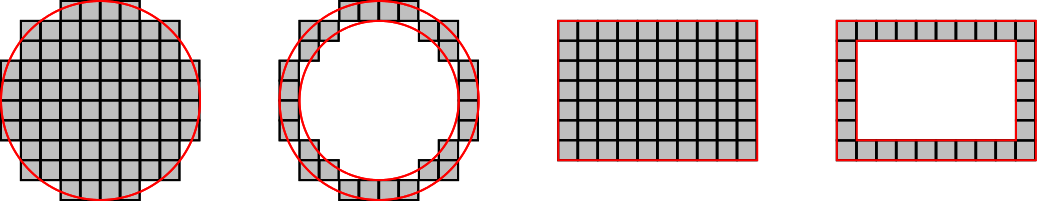
\includegraphics[scale=0.27]{./images/compartmentTypes.png}
 % compartmentTypes.png: 1042x202 pixel, 51dpi, 52.10x10.10 cm, bb=0 0 1477 286
 \caption{2D compartment types (open and solid)}
 \label{fig:compartmentTypes}
\end{figure}



The syntax to specify predefined compartments is the same as above, except that one needs to specify the type of compartment and provide the necessary arguments.
\begin{bnfsource}
'\%compartment:' name=id type=id ('[' INT ']')*
\end{bnfsource}
\newpage

This is best seen with examples:
\begin{kappasource}
### 2D Shapes

%compartment: solidRectangle              [10][5]        # [height][width]
%compartment: openRectangle OpenRectangle [10][5] [2]    # [height][width] [thickness]
%compartment: solidCircle   SolidCircle   [10]           # [diameter]
%compartment: openCircle    OpenCircle    [10] [2]       # [diameter] [thickness]

### 3D Shapes

%compartment: solidCuboid                 [10][5][8]     # [height][width][depth]
%compartment: openCuboid    OpenCuboid    [10][5][8] [2] # [height][width][depth] [thickness]
%compartment: solidSphere   SolidSphere   [10]           # [diameter]
%compartment: openSphere    OpenSphere    [10] [2]       # [diameter] [thickness]
%compartment: solidCylinder SolidCylinder [10][8]        # [diameter][length]
%compartment: openCylinder  OpenCylinder  [10][8] [2]    # [diameter][length] [thickness]
\end{kappasource}



\subsection{Channels}\label{Chan}

%\todr{As an invariant of motion? do dynamic channel preserve static ones? is there a complete partition between static/dynamic channels? does a channel need to have a 1-1 map between lhs voxels and rhs ones? Yes! How is the matching done - using agent groups?} 

The structure of a compartment is complemented by the definition of \emph{channels} which define how voxels are linked within and across compartments. Channels are used in defining both static links between agents in different voxels, and the motion of agents through the geometry of the model. The syntax is as follows:
\begin{bnfsource}
'\%channel:' id channel 
| '\%channel:' id '(' channel ')' ('+' '(' channel ')')*
\end{bnfsource}
where
\begin{bnfsource}
channel :
  source=locations '->' target=locations

locations :
  location (',' location)*
\end{bnfsource}
Where \verb|location| is as described above. For example:
\begin{kappasource}
\%compartment: torus [10][200]    # 10x200 voxels in size

# Link all voxels to their horizontally adjacent neighbours
# Link all voxels to their vertically adjacent neighbours
# Wrap around the voxels on the left and right edges to create a cylinder
# Wrap around the voxels on the top and bottom edges to create a torus
\%channel: meshlinks {\textbackslash}
    (:torus[x][y] -> :torus[x +1][y]) + (:torus[x][y]   -> :torus[x -1][y]) + {\textbackslash}
    (:torus[x][y] -> :torus[x][y +1]) + (:torus[x][y]   -> :torus[x][y -1]) + {\textbackslash}
    (:torus[0][y] -> :torus[9][y])    + (:torus[9][y]   -> :torus[0][y])    + {\textbackslash}
    (:torus[x][0] -> :torus[x][199])  + (:torus[x][199] -> :torus[x][0])
\end{kappasource}

The above code defines a thin torus composed of a 2D mesh. (Note the use of \Verb+\+ to extend a command beyond a line.)

Locations on the left hand side (lhs) of the channel definitions above may contain either constant values or single variable names; complex expressions are forbidden and repeated variables are ignored and treated as new ones. The variable names are used to define the dimensions which will be iterated through to produce links. Locations on the right hand side (rhs) allow constant values or complex expressions involving the variables defined on the left hand side of the expression. It is invalid for the rhs to use variables not defined in the lhs. If setting the values of variables references valid voxels on both the left and right, then those voxels are deemed to be linked. References to voxels \emph{outside} the dimensions of the compartment are ignored, and no link is created. Locations referenced in a channel definition can belong to the same compartment, thus defining an intra-compartment channel, or to different compartments. The modulus operator \Verb+%+ 
is useful in defining repeated patterns of linkage within a compartment, for example the 2D hexagonal mesh described in Appendix \ref{sec:spatialPatterns}.

Channels can make use of multiple source voxels simultaneously. For example if a model was to represent the movement of transmembrane proteins laterally along the surface of a membrane, then the channel used to describe the lateral motion would need to include simultaneous movement in two compartments (cytosol and membrane). This is represented as follows:

\begin{kappasource}
\%compartment: membrane [5][5]
\%compartment: cytosol  [5][5][5]

\%channel: diffusion {\textbackslash}
    (:membrane [x][y], :cytosol [u][v][0] -> :membrane [x +1][y], :cytosol [u +1][v][0]) + {\textbackslash}
    (:membrane [x][y], :cytosol [u][v][0] -> :membrane [x -1][y], :cytosol [u -1][v][0]) + {\textbackslash}
    (:membrane [x][y], :cytosol [u][v][0] -> :membrane [x][y +1], :cytosol [u][v +1][0]) + {\textbackslash}
    (:membrane [x][y], :cytosol [u][v][0] -> :membrane [x][y -1], :cytosol [u][v -1][0])
\end{kappasource}

Here, variables \Verb+x+, \Verb+y+ represent locations in the membrane, and \Verb+u+, \Verb+v+ represent locations in the top layer of the cytosol. The definition updates the locations in these two compartments in unison, resulting in the declaration of $5^4$ different 2-input channels. Note that there must be the same number of voxels in the source and target of a channel (two in this example), and thus, channels define a one-one mapping between source and target voxels.

%\todr{because of the intention of `moving simultaneously' this can only mean that u=x,v=y but it is incomprehensible; no! x,y,u,v are anything; created channels which will be only used vertically, ie x=u, v=y by restriction through a static link; you can make u=x, v=y if you want but that is ignored see above}

Further examples of compartment and channel specifications for common structures are given in Appendix~\ref{sec:spatialPatterns}.

\subsubsection{Predefined channel types}\label{predefCtype}

Commonly used 2- and 3-dimensional channel types can be concisely defined. 

\medskip 
\begin{table}[h!]
\centering
\topcaption{Predefined channels.\label{predefchan}}
\begin{tabular}{|l|l|}
\hline
Name & \multicolumn{1}{|c|}{Each voxel connected to}\\ 
\hline
\multicolumn{2}{|c|}{2D}\\
\hline
EdgeNeighbour & 4 neighbours which share an edge in grid \\
Hexagonal & 6 neighbours which share an edge in hexagonal grid \\
Neighbour & 8 neighbours which share an edge or corner in grid \\
\hline
\multicolumn{2}{|c|}{3D}\\
\hline
FaceNeighbour & 6 neighbours which share a face in grid\\
Neighbour & 26 neighbours which share a face, edge or corner in grid \\
\hline
\end{tabular} 

\end{table}


\medskip 

\begin{figure}[h!]
 \centering
 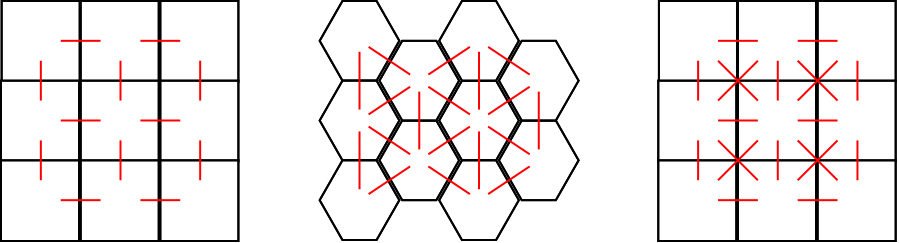
\includegraphics[scale=0.31]{./images/channelTypes.png}
 % channelTypes.png: 1042x202 pixel, 51dpi, 52.10x10.10 cm, bb=0 0 1477 286
 \caption{2D channel types: EdgeNeighbour, Hexagonal and Neighbour}
 \label{fig:channelTypes}
\end{figure}

There are also predefined directional channel types usable in both 2D and 3D compartments

\medskip

\begin{tabular}{|c|l|}
\hline
Name & \multicolumn{1}{|c|}{Each voxel connected to}\\ 
\hline
Radial & neighbours both directly towards and away from compartment centre  \\
RadialIn & neighbours both directly towards compartment centre \\
RadialOut & neighbours both directly away from compartment centre \\
Lateral & neighbours at same distance from compartment centre \\
\hline
\end{tabular} 

\medskip 

\begin{figure}[h!]
 \centering
 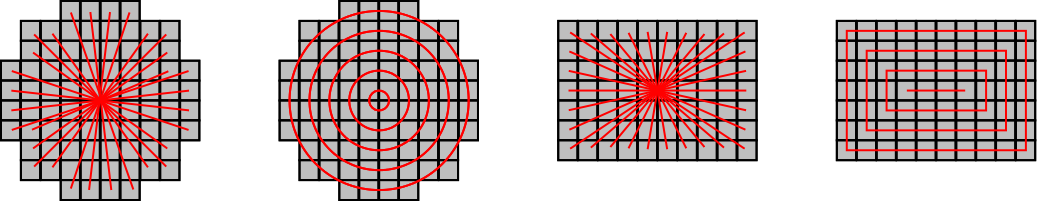
\includegraphics[scale=0.27]{./images/directedChannelTypes.png}
 % directedChannelTypes.png: 1042x202 pixel, 51dpi, 52.10x10.10 cm, bb=0 0 1477 286
 \caption{Directed channel types: Radial and Lateral}
 \label{fig:directedChannelTypes}
\end{figure}

The syntax to use a predefined channel type is

\begin{bnfsource}
'\%channel:' id channel
| '\%channel:' id '(' channel ')' ('+' '(' channel ')')*
\end{bnfsource}
where
\begin{bnfsource}
channel :
  type=id source=locations '->' target=locations
\end{bnfsource}
Where \verb|locations| is as described above. For example:
\begin{kappasource}
\%compartment: solidRectangle[5][5] # [height][width]

\%channel: radial Radial :solidRectangle -> :solidRectangle
\%channel: radialIn RadialIn :solidRectangle -> :solidRectangle
\%channel: radialOut RadialOut :solidRectangle -> :solidRectangle
\%channel: lateral Lateral :solidRectangle -> :solidRectangle
\end{kappasource}

\subsubsection{Using predefined channel types between compartments}

It is possible to use predefined channel types (usually `Neighbour' see also Table \ref{predefchan}) to describe movement between compartments. For this to be valid, the compartments must have compatible geometry. Compatible compartments are treated as being nested one inside the other and the channel then specifies the diffusion (or agent linkage) across the boundary between the two compartments. The compartments must fit together exactly, with no overlapping voxels or gaps. For example, a circle may only be nested inside a larger open circle whose dimensions (diameter and thickness) allow the smaller circle to fit exactly inside.

\begin{kappasource}
\%compartment: cytosol   SolidCircle   [3]           # [diameter]
\%compartment: membrane  OpenCircle    [7] [2]       # [diameter] [thickness]

\%channel: domainLink Neighbour (:cytosol -> :membrane) + (:membrane -> :cytosol)
\end{kappasource}


\subsection{Locating agents}

The definitions above can now be used to locate species within the model. Any rule or directive (i.e., variables, observables, and initial conditions) that accepts agents as part of its definition, now allows these agents to be located. For each group of agents, a prefixed location constrains the agents to that location. For example: 

%\tod{what is a group of agents? all examples below are single agents. What does evenly distributed mean? random? or really even - which is not always possible}

\begin{kappasource}
\%compartment: membrane [5][5]
\%compartment: cytosol  [5][5][5]

\%init: 1000 A                   # A distributed evenly among all voxels in model 
\%init: 1000 :cytosol B          # B distributed evenly among all voxels in cytosol
\%init: 1000 :membrane[2][2] C   # C in one voxel of the membrane only 
\end{kappasource}

In addition, individual agents can have a specified location. For example:
\begin{kappasource}
\%init: 1000 B:cytosol             # B distributed evenly among all voxels in cytosol
\%init: 1000 C:membrane[2][2](s~u) # C in one voxel of the membrane only 
\end{kappasource}

(Saying that $n$ copies of \Verb+A+ are evenly distributed among a set of $N$ voxels, means that all voxels receive the same number of \Verb+A+s, i.e.\ the quotient of $n$ by $N$, the remainder being allocated randomly.)

When locations are specified both for agent groups and individual agents, the individual agent location takes precedence. This allows for concise definition of agent groups where all but one of the agents in the group share a location.

Voxel wildcards may also be used when specifying agent location. For example:

\begin{kappasource}
\%compartment: cytosol [5][5][5]

\%init: 1000 :cytosol[5][5][?] A # A distributed along a single edge of compartment
\%init: 1000 :cytosol[?][?][2] B # B distributed in a plane across middle of compartment
\end{kappasource}


\subsection{Agent links}

Agents in neighbouring voxels can be linked together provided their voxels are linked by a defined channel. This is an extension of the basic Kappa link syntax to name the channel used to link the agents. For example:

\begin{kappasource}
\%compartment: membrane [5][5]
\%compartment: cytosol  [5][5][5]

\%channel: domainLink {\textbackslash}
    (:membrane [x][y] -> :cytosol [x][y][0]) + (:cytosol [x][y][0] -> :membrane [x][y])

\%init: 1000 A:membrane(d!1:domainLink), B(d!1)
\end{kappasource}

The above describes a model where the species \Verb+AB+ exists in two compartments, \Verb+B+ in the cytosol and \Verb+A+ embedded in the membrane. When specifying agent links using channels, only one end of the link needs to specify the channel. If a link does not specify the channel, it is assumed that both agents party to the link exist in the \emph{same} voxel.

Links including channels can be created or broken in the same way as basic Kappa links in  rules.

\subsection{Species movement}

Species can move along defined channels. Movement transition rules can either constrain the movement by species chosen, or by source location.  Species movement is described using the \verb|->:| operator. 

\begin{bnfsource}
(source=location)? '->:' channelName=id (target=location)?
|  (a=agentGroup)? '->:' channelName=id (b=agentGroup)?
\end{bnfsource}

For example: 

\begin{kappasource}
\%compartment: membrane [5][5]

\%channel: diffusion {\textbackslash}
    (:membrane [x][y] -> :membrane [x+1][y]) + (:membrane [x][y] -> :membrane [x - 1][y]) + {\textbackslash}
    (:membrane [x][y] -> :membrane [x][y+1]) + (:membrane [x][y] -> :membrane [x][y - 1])

'diffusion A' A(s,t) ->:diffusion A(s,t) @ 1.0
'diffusion B' B(s,t) ->:diffusion B(s,t) @ 1.0
'diffusion AB' A(s!1,t),B(s!1,t) ->:diffusion A(s!1,t),B(s!1,t) @ 0.5

'diffusion all' ->:diffusion @ 1.0 # All species located in a single voxel will match this rule
\end{kappasource}

To describe movement of species which span more than one voxel, one can use the multiple source channel definition given above (\S\ref{Chan}):

\begin{kappasource}
\%compartment: membrane [5][5]
\%compartment: cytosol  [5][5][5]

\%channel: diffusion {\textbackslash}
    (:membrane [x][y], :cytosol [u][v][0] -> :membrane [x+1][y],  :cytosol [u+1][v][0])  + {\textbackslash}
    (:membrane [x][y], :cytosol [u][v][0] -> :membrane [x -1][y], :cytosol [u -1][v][0]) + {\textbackslash}
    (:membrane [x][y], :cytosol [u][v][0] -> :membrane [x][y+1],  :cytosol [u][v+1][0])  + {\textbackslash}
    (:membrane [x][y], :cytosol [u][v][0] -> :membrane [x][y -1], :cytosol [u][v -1][0])

\%channel: domainLink {\textbackslash}
    (:membrane [x][y] -> :cytosol [x][y][0]) + (:cytosol [x][y][0] -> :membrane [x][y])

'diffusion A' A_m:membrane(s,t,d!1:domainLink),A_c(d!1) ->:diffusion {\textbackslash}
              A_m:membrane(s,t,d!1:domainLink),A_c(d!1) @ 1.0
              
'diffusion B' B_m:membrane(s,t,d!1:domainLink),B_c(d!1) ->:diffusion {\textbackslash}
              B_m:membrane(s,t,d!1:domainLink),B_c(d!1) @ 1.0

'diffusion AB' A_m:membrane(s!2,t,d!1:domainLink),A_c(d!1), {\textbackslash}
               B_m:membrane(s!2,t,d!3:domainLink),B_c(d!3) ->:diffusion {\textbackslash}
               A_m:membrane(s!2,t,d!1:domainLink),A_c(d!1), {\textbackslash}
               B_m:membrane(s!2,t,d!3:domainLink),B_c(d!3) @ 0.5
\end{kappasource}

\subsubsection{Fixed location constraints}

It is necessary in some models to distinguish between species which can diffuse freely within all voxels of a compartment, and species which are fixed to a single voxel. The predefined location \verb|:fixed|, used on the right hand side of a transition rule, allows this. For example, in the model below, agent \verb|A()| can diffuse freely, while agent \verb|B()| must remain static. 

\begin{kappasource}
\%compartment: cytosol [5][5][5]

\%channel: diffusion Neighbour :cytosol -> :cytosol

'diffusion A' :cytosol A(),B() ->:diffusion :cytosol A(),B:fixed() @ 1.0
\end{kappasource}


\subsection{Instance specific reaction rates}

The rate of a transition rule can depend on the composition and size of the particular species it is being applied to. This is possible for all types of transition, not just diffusion transitions.  

An agent description enclosed in \Verb+||+ may be used in a rate equation.

\begin{bnfsource}
'|' agentGroup '|'
\end{bnfsource}

where \verb|agentGroup| is agent definition syntax as used on the left hand side of transition rules.

When applied to particular instances of complexes, the number of matching agent structures in the complex instances chosen are counted and substituted into the rate.

For example, in the model below, diffusion rate is inversely proportional to the number of \verb|A()| in the chosen complex

\begin{kappasource}
\%compartment: array [10]
\%channel: diffusion :array[x] -> :array[x+1]

\%agent: A(x,y)

\%init: 100 :array[0] A(x,y!1), A(x!1,y!2), A(x!2,y!3), A(x!3,y)
\%init: 100 :array[0] A(x,y!1), A(x!1,y)
\%init: 100 :array[0] A(x,y)

'diffusion A' A(x) ->:diffusion A(x) @ 1 / |A()|
\end{kappasource}

In the second example, the diffusion rate depends on the agent types within individual complex instances

\begin{kappasource}
\%compartment: array [10]
\%channel: diffusion :array[x] -> :array[x+1]

\%agent: A(x,y)
\%agent: B(x,y)

\%init: 100 :array[0] A(x,y!1), A(x!1,y!2), A(x!2,y!3), A(x!3,y)
\%init: 100 :array[0] A(x,y!1), A(x!1,y!2), B(x!2,y!3), B(x!3,y)
\%init: 100 :array[0] B(x,y!1), B(x!1,y!2), B(x!2,y!3), B(x!3,y)
\%init: 100 :array[0] B(x,y!1), B(x!1,y!2), A(x!2,y!3), A(x!3,y)

'diffusion AX' A(x) ->:diffusion A(x) @ 1 / (|A()| + 10 * |B()|)
'diffusion BX' B(x) ->:diffusion B(x) @ 1 / (|A()| + 10 * |B()|)
\end{kappasource}

In the final example, the diffusion rate depends on the states of the agents within individual complex instances

\begin{kappasource}
\%compartment: array [10]
\%channel: diffusion :array[x] -> :array[x+1]

\%agent: A(x,y,s~y~n)

\%init: 100 :array[0] A(s~y,x,y!1), A(s~y,x!1,y!2), A(s~y,x!2,y!3), A(s~y,x!3,y)
\%init: 100 :array[0] A(s~y,x,y!1), A(s~y,x!1,y!2), A(s~n,x!2,y!3), A(s~n,x!3,y)
\%init: 100 :array[0] A(s~n,x,y!1), A(s~n,x!1,y!2), A(s~n,x!2,y!3), A(s~n,x!3,y)
\%init: 100 :array[0] A(s~n,x,y!1), A(s~n,x!1,y!2), A(s~y,x!2,y!3), A(s~y,x!3,y)

'diffusion A' A(x) ->:diffusion A(x) @ 1 / (|A(s~y)| + 10 * |A(s~n)|)
\end{kappasource}

The \Verb+||+ clause allows any agent declaration that could appear on the left hand side of a transition rule, including agents, complexes, agent state and agent location.

\subsection{Voxel breakdown of observables}

Observables using the constructs \verb|%obs:| and \verb|%var:| can be used to get the total amount of species per compartment. For example:

\begin{kappasource}
\%obs: 'A in cytosol' :cytosol A()
\%var: 'A in cytosol' :cytosol A()
\end{kappasource}

However, for some simulations, recording the value of observables in each voxel of a compartment is useful. In these cases, using the keyword \verb|voxel| will allow recording of observables per voxel. This works only on observable or variable declarations which specify a compartment as the location of the declaration. For example:

\begin{kappasource}
\%obs: voxel 'A in cytosol' :cytosol A()
\%var: voxel 'A in cytosol' :cytosol A()
\end{kappasource}

The above each declare variables which record for each voxel within the compartment \verb|cytosol|.

\tbf{Warning} - as all voxels within the compartment are recorded for each observable using the \verb|voxel| keyword at each timepoint, the output data file will rapidly become very large.

\bigskip For example models demonstrating the use of the language extensions, refer to Appendix \ref{chap:resources}.

%\newpage
%
%\chapter{Spatial Kappa simulator User Guide}

\section{Obtaining the simulator}

The simulator is available from GitHub as the source Eclipse project, or as a single executable jar file. Both are available at \url{https://github.com/donal-s/SpatialKappa/downloads}. The simulator in its current state was optimised specifically for the 2010 Edinburgh iGEM project. This is apparent mostly in the design of the compartment view pane. Extending this view for more generic use is a planned extension.

\section{Starting the simulator}

\subsection{Running the executable jar}

The simulator can be started by running the executable jar file:\\
\verb|java -jar SpatialKappa-v1.0.0.jar|\\\\
Double clicking the jar file usually works too.

\subsection{Running from the Eclipse project}

The main class of the simulator is \\
\verb|org.demonsoft.spatialkappa.ui.TransitionMatchingSimulatorGui|\\\\
Running as a Java Application will bring up the simulator.


\section{Using the simulator}


The initial screen appears as figure \ref{fig:startup}.

\begin{figure}[h!]
 \centering
 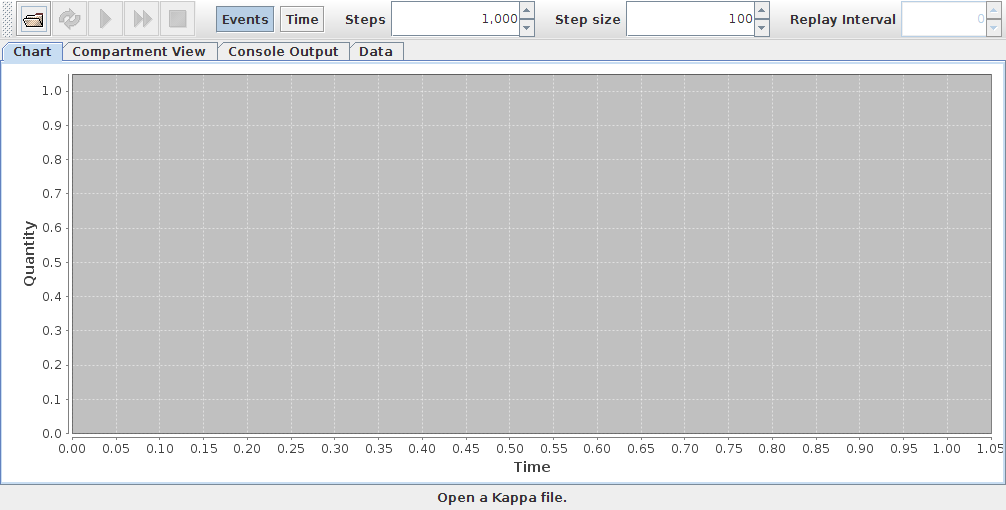
\includegraphics[scale=0.3]{./images/startup.png}
 % startup.png: 1006x510 pixel, 72dpi, 35.49x17.99 cm, bb=0 0 1006 510
 \caption{Initial view}
 \label{fig:startup}
\end{figure}

The toolbar options are:

\begin{tabular}{cl}
 
\includegraphics[scale=0.5]{./images/Open.png} & Open a Kappa or Kappa replay file \\
 
\includegraphics[scale=0.5]{./images/Reopen.png} & Reopen the current file  \\
 
\includegraphics[scale=0.5]{./images/Run.png} & Run the current file \\
 
\includegraphics[scale=0.5]{./images/Replay.png} & Replay the current replay file or last run \\
 
\includegraphics[scale=0.5]{./images/Stop.png} & Stop the currently running simulation \\
 
\includegraphics[scale=0.5]{./images/EventsOrTime.png} & Choose event or time based simulation \\
\end{tabular}

\subsection{Opening a Kappa or Kappa replay file}

Select the 'Open' button on the toolbar and select the file to open. The current implementation expects Kappa source files to have the suffix \verb|.ka| and Kappa replay files (discussed later) to have the suffix \verb|.kareplay|. If the file is parsed successfully, a summary of the Kappa model is displayed in the 'Data' pane (see figure \ref{fig:dataPane}). 

\begin{figure}[h!]
 \centering
 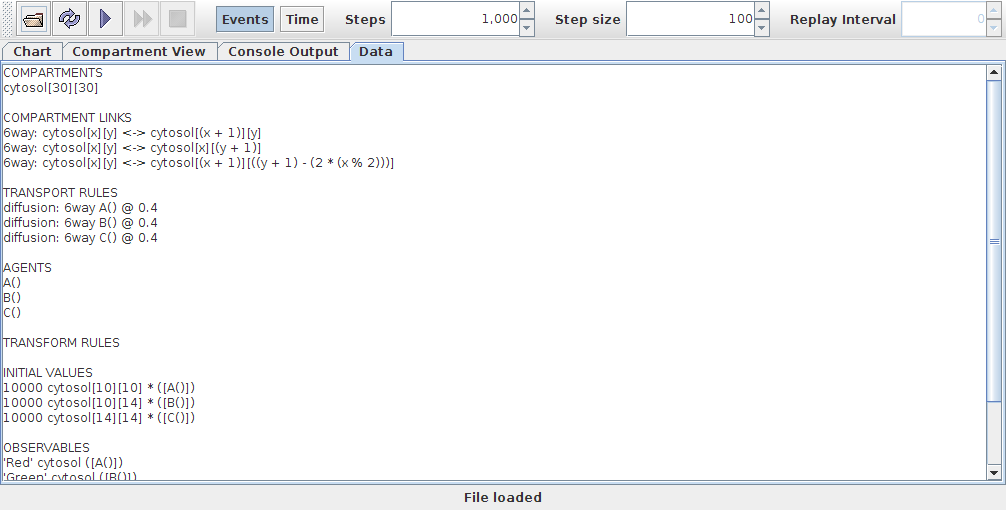
\includegraphics[scale=0.3]{./images/FileOpenDataPane.png}
 % FileOpenDataPane.png: 1006x510 pixel, 72dpi, 35.49x17.99 cm, bb=0 0 1006 510
 \caption{Data pane showing loaded Kappa model}
 \label{fig:dataPane}
\end{figure}

Any errors in reading the Kappa file are shown in the 'Console Output' pane.

The currently open Kappa file can be refreshed from disk by selecting the 'Reopen' button. Useful when editing the Kappa model.

\subsection{Running a simulation}

With a successfully opened Kappa model, one can run a simulation by selecting the 'Run' button. Simulation parameters can be set on the toolbar before running. There is the option to do an event or a time based simulation. For an event based simulation, the number of steps for the simulation (i.e. data points on the time series chart), and the number of finite rate events per step can be set. Equivalent options for time based simulation can also be set.

The simulation can be halted at any point by selecting the 'Stop' button. Note that complex simulations may take a while to start up while data structures are being generated.

\subsection{Running a simulation replay}

As the simulation runs, the state of the simulation observables are logged to disk in a replay file after every step. Once the simulation is complete, this replay file can be rerun by selecting the 'Replay' button. The 'Replay Interval' field allows a delay (in ms) to be added between each step.

Note - the current storage format is binary, and version dependent. Creation of a more permanent trace storage format is a planned enhancement.


\section{Spatial visualisation tools}

While the raw data produced from simulations is useful, visualisation of the data is important. There are a couple of simple visualisation panels in the simulator. These are dynamically updated as the simulation runs to give the user an idea of how the simulation is progressing. They are however basic in comparison to some of the commercial simulation data visualisation tools available.

The excellent JFreeChart \citep{JFreeChartwebsite} library was used for generating the charting components. Both charts have formatting and save capability, and the time series panel is zoomable.

\subsection{Time series chart}

This chart is similar to the standard Gnuplot output from Simplx. It is a line graph showing observable quantity against time for all observable definitions in the model.

\begin{figure}[h!]
 \centering
 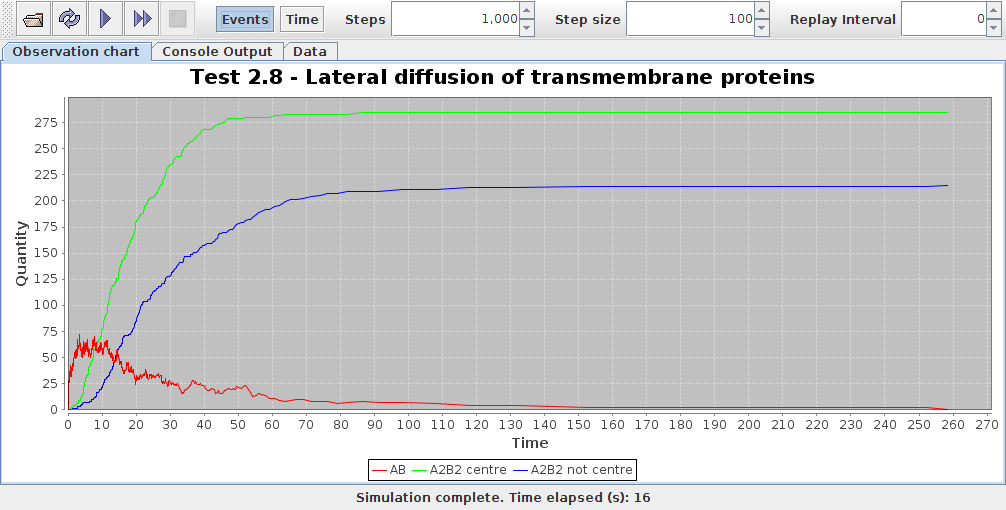
\includegraphics[scale=0.3]{./images/ChartPane.png}
 % ChartPane.png: 1006x510 pixel, 72dpi, 35.49x17.99 cm, bb=0 0 1006 510
 \caption{Sample time series chart output}
 \label{fig:chartPane}
\end{figure}

\subsection{Compartment chart}

This view allows more detailed visualisation of the transport of a species within the cells of a single compartment. It can show local positive feedback sites, or diffusion of a species through a compartment. There are a couple of visualisation options which can be selected at runtime to tailor the output.

Note that the current implementation is designed to view a 3-channel hexagonal mesh, and that view works only for observations labelled \verb|'Red'|, \verb|'Blue'| and \verb|'Green'| in a compartment labelled \verb|'Cytosol'|. Making this more generic is also a planned area for extension.

\begin{figure}[h!]
 \centering
 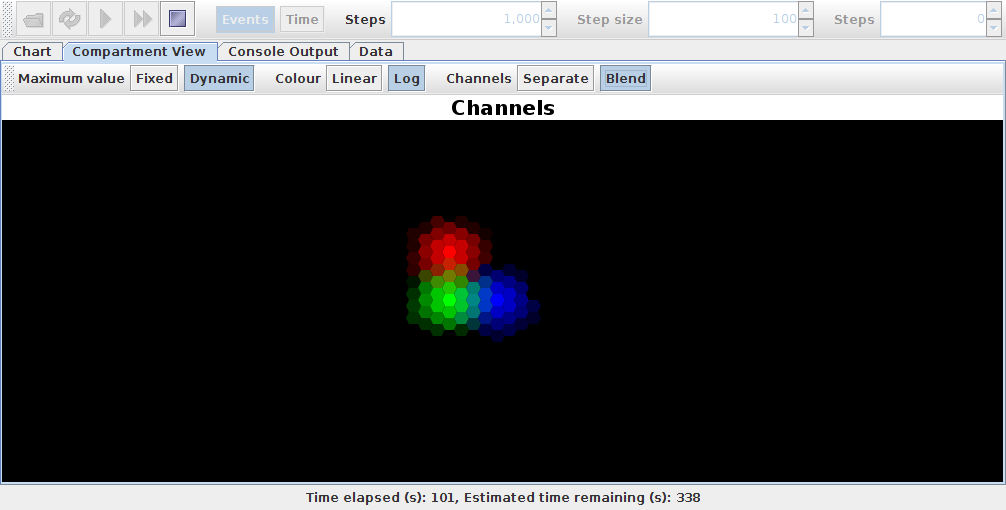
\includegraphics[scale=0.3]{./images/CompartmentView.png}
 % CompartmentView.png: 1006x510 pixel, 72dpi, 35.49x17.99 cm, bb=0 0 1006 510
 \caption{Sample compartment chart output}
 \label{fig:compartmentPane}
\end{figure}


\chapter{Spatial Kappa simulator User Guide}

\section{Obtaining the simulator}

The simulator is available from GitHub as the source Eclipse project, or as a single executable jar file. Both are available at \url{https://github.com/lptolik/SpatialKappa/}. 

\section{Starting the simulator}

\subsection{Running the executable jar}

The simulator can be started by running the executable jar file:\\
\verb|java -jar SpatialKappa-v2.1.1.jar|\\\\
Double clicking the jar file usually works too.

\subsection{Running from the Eclipse project}

The main class of the simulator is \\
\verb|org.demonsoft.spatialkappa.ui.SpatialKappaSimulator|\\\\
Running as a Java Application will bring up the simulator.


\section{Using the simulator}

The initial screen appears as figure \ref{fig:startup}.

\begin{figure}[h!]
 \centering
 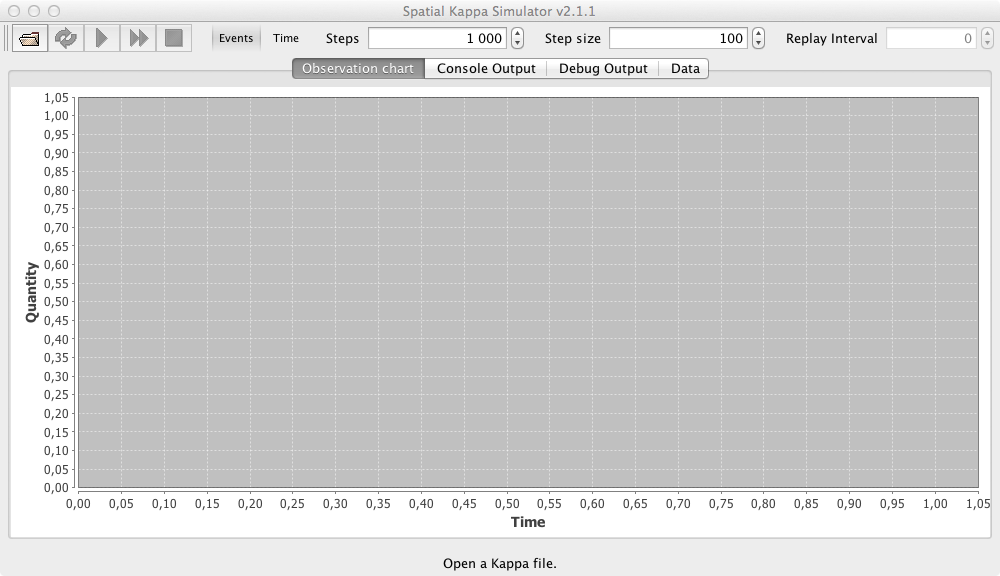
\includegraphics[scale=0.45]{./images/startup2.png}
 % startup.png: 1006x510 pixel, 72dpi, 35.49x17.99 cm, bb=0 0 1006 510
 \caption{Initial view}
 \label{fig:startup}
\end{figure}

The toolbar options are:

\begin{tabular}{cl}
 
\includegraphics[scale=0.5]{./images/Open.png} & Open a Kappa or Kappa replay file \\
 
\includegraphics[scale=0.5]{./images/Reopen.png} & Reopen the current file  \\
 
\includegraphics[scale=0.5]{./images/Run.png} & Run the current file \\
 
\includegraphics[scale=0.5]{./images/Replay.png} & Replay the current replay file or last run \\
 
\includegraphics[scale=0.5]{./images/Stop.png} & Stop the currently running simulation \\
 
\includegraphics[scale=0.5]{./images/EventsOrTime.png} & Choose event or time based simulation \\
\end{tabular}

\subsection{Opening a Kappa or Kappa replay file}

Select the `Open' button on the toolbar and select the file to open. The current implementation expects Kappa source files to have the suffix \verb|.ka| and Kappa replay files (discussed later) to have the suffix \verb|.kareplay|. If the file is parsed successfully, a summary of the Kappa model is displayed in the `Data' pane (see figure \ref{fig:dataPane}). 

\begin{figure}[h!]
 \centering
 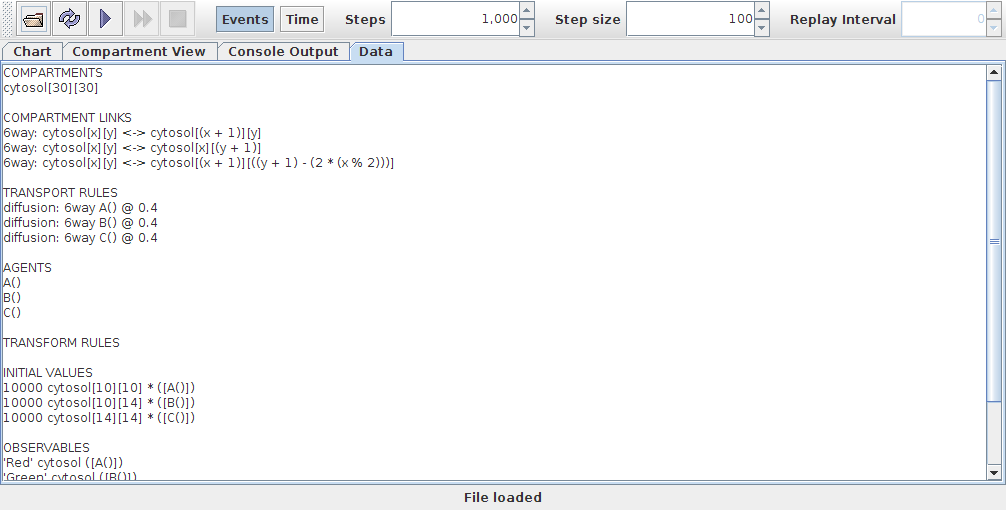
\includegraphics[scale=0.45]{./images/FileOpenDataPane.png}
 % FileOpenDataPane.png: 1006x510 pixel, 72dpi, 35.49x17.99 cm, bb=0 0 1006 510
 \caption{Data pane showing loaded Kappa model}
 \label{fig:dataPane}
\end{figure}

Any errors in reading the Kappa file are shown in the `Console Output' pane.

The currently open Kappa file can be refreshed from disk by selecting the `Reopen' button. Useful when editing the Kappa model.

\subsection{Running a simulation}

With a successfully opened Kappa model, one can run a simulation by selecting the `Run' button. Simulation parameters can be set on the toolbar before running. There is the option to do an event or a time based simulation. For an event based simulation, the number of steps for the simulation (i.e. data points on the time series chart), and the number of finite rate events per step can be set. Equivalent options for time based simulation can also be set.

The simulation can be halted at any point by selecting the `Stop' button. Note that complex simulations may take some time to start up while data structures are being generated.

A replay file of the simulation is created in the same directory as the Kappa model. The file format is similar to that produced by KaSim.

\subsection{Running a simulation replay}

As the simulation runs, the state of the simulation observables are logged to disk in a replay file after every step. Once the simulation is complete, this replay file can be rerun by selecting the `Replay' button. The `Replay Interval' field allows a delay (in ms) to be added between each step.

The file format is similar to that produced by KaSim. Renaming KaSim data output to have the suffix \verb|.kareplay| will allow KaSim output to also be visualised using this tool.

\section{Time series chart}

%While the raw data produced from simulations is useful, visualisation of the data is important. 
There is a simple visualisation panel in the simulator. This is dynamically updated as the simulation runs to give the user an idea of how the simulation is progressing. It is however basic in comparison to some of the commercial simulation data visualisation tools available.

The time series chart is similar to the standard Gnuplot output from KaSim. It is a line graph showing observable quantity against time for all observable definitions in the model. The excellent JFreeChart \citep{JFreeChartwebsite} library was used for generating the charting component. The chart has formatting and save capability, and is zoomable.

\begin{figure}[h!]
 \centering
 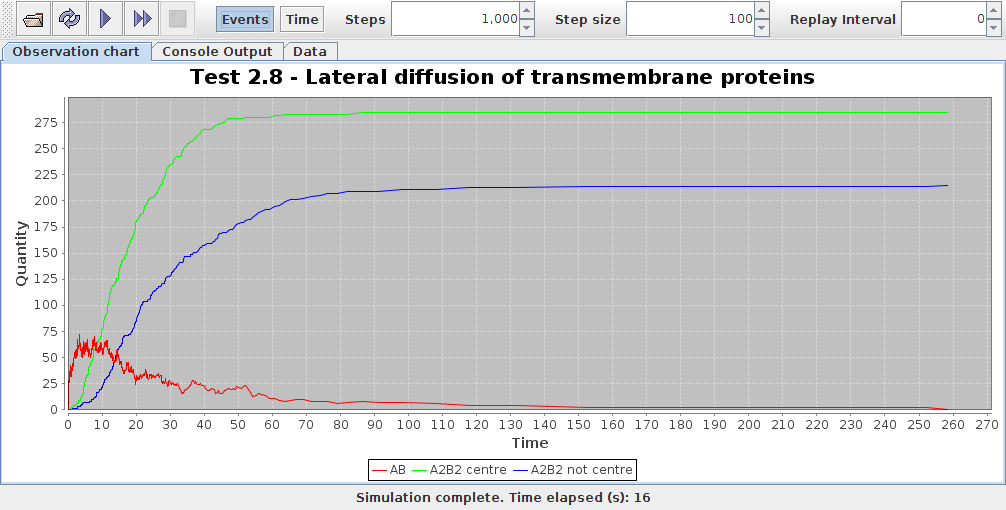
\includegraphics[scale=0.4]{./images/ChartPane.png}
 % ChartPane.png: 1006x510 pixel, 72dpi, 35.49x17.99 cm, bb=0 0 1006 510
 \caption{Sample time series chart output}
 \label{fig:chartPane}
\end{figure}

%\chapter{Spatial Kappa reference implementation}

The algorithm implemented by Spatial Kappa simulator is similar to one described in \cite{Elf:2004fv}. In this chapter we briefly outlined main steps of the Spatial Kappa simulator algorithm.

Apart from the differences accounted for the rule-based nature of the Spatial Kappa simulator, the major difference between our algorithm and the classical Next Subvolume algorithm is that there there is no difference between application of the reaction event and diffusion event. The reason for different treatment of diffusion events in the original algorithm was the optimisation of the performance: type of event defined one or two voxel states has to be updated. With introduction of multi compartmental complexes the benefit of different treatment has disappeared, so in Spatial Kappa all events are equal in terms of Gillespie algorithm. 

\section{Initialization}
Kappa language grammar and the Spatial Kappa extension are defined with ANTLR 3.0 parser generation framework (see also Appendix \ref{chap:spatialGrammar}). The grammar definition allows to perform number of initialization steps during the parsing phase, but most initialisation performed by simulator itself.

Rule-based nature of the simulator allows to avoid some steps of initialisation, for example, there is no need for connectivity matrix. The channel definitions would play a role of rules defining diffusion reactions in the same way as reaction rules replace reaction definitions.

The main task of initialisation step is the distribution of agents and complexes between voxels. There are two options to do this: model can define exact number of agents and complexes in particular voxel, or total amount of agents in the system. In the later case simulator will distribute agents homogeneously among all voxels of the system.

The next initialisation step is to define possible applications of the reaction and diffusion rules based upon initial state of the system. In this step we need to calculate all possible mappings between rule left-hand-sides and system state and calculate activities for each of that mappings. The activity of the rule is the sum of activities of each of its mappings. Activities for all rules that has no mappings to the state of the system are set to zero.

\section{Main simulation loop}
The main simulation loop of the Spatial Kappa simulator is the same as in Next Subvolume algorithm with modifications due to rule-based nature of the model definition. There are two types of model declarations that need to be processed before ordinary rules: perturbations and infinite rate rules.

\subsection{Perturbations}
Perturbation is a standard Kappa language construct that allow model to change its state when special firing conditions are met. For example, add drug to the system at particular time point, or open the ion channel when transmembrane potential reach some value. In the Spatial Kappa simulator perturbation are checked first in the main simulation loop and if firing conditions are met then modifications to the system state are applied.

\subsection{Infinite rate rules}
It is possible to set the rate constant of rule to infinity in Spatial Kappa model. For example to compare Spatial Kappa model with ordinary Kappa model we could set infinity rate to all diffusion rules. Rules which has rate constants specified by equation could get infinity rate after application of the equation to the system state. It is obvious that infinite rate rules requires special treatment as their application do not progress the system time. In the Spatial Kappa simulator infinite rate rules are applied to the system after perturbation check until either no rules left or state of the system change too much. Application of the infinite rate rule is similar to the finite rate rule, it just do not change the system time, but due to the way they are applied infinite rate rules could significantly slow down the simulation.

\subsection{Finite rate rules}
After application of  infinite rate rules system pick one of the rules and one of that rule mappings and apply it to the system. The process of selection of the rule and one of its mapping is the same as in Next Subvolume method: simulator calculates total activity $r_{tot}=\sum_{i}{r_{i}}$ or $m_{tot}^{i}=\sum_{j}{m_{j}^{i}}$ and generate random number $rand$ uniformly distributed between 0 and 1. Choose rule (mapping) if $rand < r_{i}/r_{tot}$ ($rand < m_{j}^{i}/m_{tot}^{i}$) to pick the rule (mapping) for application.

After rule application simulator change the state of the system according to the rule right-hand-side, progress the system time by the same $\Delta\tau$ as in Next Subvolume method and recalculate the rule mappings and their activities.



\chapter{Spatial Kappa reference implementation}

The algorithm implemented by Spatial Kappa simulator is similar to the Next Subvolume algorithm described in Ref.~\citep{Elf:2004fv}. In this chapter we briefly outline its main steps.

Apart from the differences coming from the rule-based nature of the Spatial Kappa simulator, the major difference between our algorithm and the classicalone  is that there there is no distinction made between the application of a reaction event and a diffusion one. The reason for a different treatment of diffusion events in the original algorithm was the optimisation of performance. 
With the introduction of multi-compartmental complexes the benefit of such a different treatment has disappeared, so in Spatial Kappa all events are seen as equal in terms of the underpinning Gillespie algorithm. 

\section{Initialization}
The Kappa grammar and its spatial extension are defined within the ANTLR 3.0 parser generation framework (see also Appendix \ref{chap:spatialGrammar}). This allows one to perform a number of initialization steps during the parsing phase, but most of the initialization rests on the simulator itself.

The rule-based nature of the framework allows to avoid some steps of initialization, for example, there is no need to build a connectivity matrix between voxels. The channel definitions play the role of rules defining diffusion reactions, 
in the same way as transform rules replace reaction definitions.

The first main task of the initialization is the \emph{distribution} of agents and complexes between voxels. There are two options to do this: the model may define the exact number of agents and complexes in a particular voxel, or the total amount of agents in a compartment. In the latter case, the simulator will distribute agents homogeneously among all the compartment voxels.

The second important initialization step is to record the possible applications of reaction and diffusion rules based on the initial state. In this step one needs to calculate all possible mappings between rule left-hand-sides and the system state (a.k.a., all matchings) and their activities. The activity of the rule is the sum of activities of each of its mappings. (Rules with no mappings have zero activity.)

\section{Main simulation loop}
The main simulation loop of the Spatial Kappa simulator is the same as in Next Subvolume algorithm with modifications due to rule-based nature of the model. There are two types of model declarations that need to be processed \emph{before} ordinary rules: perturbations and infinite rate rules.

A \emph{perturbation} is a standard Kappa language construct that allows a model to change its state when special firing conditions are met. For example, adding a drug to the system at a particular time point, or opening ion channels when a transmembrane potential reaches some value. In the Spatial Kappa simulator perturbations are checked first in the main simulation loop and, if firing conditions are met, their modifications are applied.

%\subsection{Infinite rate rules}
It is possible to set an \emph{infinite} rate constant for a rule.
% in a Spatial Kappa model. 
For example, to compare a Spatial Kappa model with an ordinary Kappa model, one can assign an infinite rate to well-chosen temporary diffusion rules (via perturbations) to `stir' the model. 
In addition, rules which have rate constants specified by a function could receive an infinite rate depending on the system state. These require special treatment as their applications do not increment the system time. In the simulator, infinite rate rules are applied to the system after perturbation check until either there are no such rules left (or the cumulated number of applications exceeds a statically defined parameter - conventionally $1000$ in the current implementation).

%Application of the infinite rate rule is similar to the finite rate rule, it just do not change the system time, but due to the way they are applied infinite rate rules could significantly slow down the simulation.

\subsection{Finite rate rules}
After exhausting infinite rate rules, the simulator picks one of the remaining rules and a mapping thereof and applies it to the system. The process of selecting the rule and its mapping is the same as in the Next Subvolume method: the simulator picks rule $r$ with a probability proportional to $r$'s activity in the current state, and selects uniformly at random a 
mapping of $r$.
% $r_{tot}=\sum_{i}{r_{i}}$ or $m_{tot}^{i}=\sum_{j}{m_{j}^{i}}$ and generate random number $rand$ uniformly distributed between 0 and 1. Choose rule (mapping) if $rand < r_{i}/r_{tot}$ ($rand < m_{j}^{i}/m_{tot}^{i}$) to pick the rule (mapping) for application.
The rule application changes the state of the system according to $r$'s right-hand-side, and time progresses by the same increment as in the Next Subvolume method. One then recalculates the new rule mappings and activities locally as in Ref.~\citep{danos2007scalable}.


\appendix

%\chapter{Spatial Kappa Grammar}
\label{chap:spatialGrammar}



The following is a cut down version of the Antlr grammar used in the Kappa simulator. The syntax has been trimmed for readability, as the original Antlr grammar has artificial constructs for dealing with left recursion, etc. It is read basically as BNF notation with assignments (\verb|variable=bnfConstruct|). The existing basic Kappa grammar is shown in \verb|black|, with the spatial constructs shown as \SaveVerb{Verb}|blue| \newbnf{\UseVerb{Verb}}. 


\begin{bnfsource}
prog :
  (line)*

line :
  agentDecl NEWLINE!
  | \newbnf{compartmentDecl NEWLINE!}
  | \newbnf{channelDecl NEWLINE!}
  | ruleDecl NEWLINE!
  | initDecl NEWLINE!
  | plotDecl NEWLINE!
  | obsDecl NEWLINE!
  | varDecl NEWLINE!
  | modDecl NEWLINE!
  | COMMENT!
  | NEWLINE!

ruleDecl :
  label? transition rate 

transition :
  \newbnf{(source=location)? CHANNEL_TRANSITION channelName=id (target=location)?}
  | \newbnf{(a=agentGroup)? CHANNEL_TRANSITION channelName=id (b=agentGroup)?}
  | (a=agentGroup)? FORWARD_TRANSITION (b=agentGroup)?
  
agentGroup :
  \newbnf{location?} agent (',' agent)*

agent :
  id \newbnf{(location)?} ('(' (agentInterface (',' agentInterface)*)? ')')?

agentInterface :
  id state? link?

state :
  '~' id

link :
  '!' INT \newbnf{(':' channelName=id)?}
  | '!' '_' \newbnf{(':' channelName=id)?}
  | '?'

rate :
  '@' varAlgebraExpr

initDecl :
  '\%init:' (INT | label) agentGroup

agentDecl :
  '\%agent:' agentName=id ('(' (agentDeclInterface (',' agentDeclInterface)*)? ')')?

agentDeclInterface :
  id state*

\newbnf{compartmentDecl :}
  \newbnf{'\%compartment:' id ('[' INT ']')*}

\newbnf{channelDecl :}
  \newbnf{'\%channel:' linkName=id channel}
  \newbnf{| '\%channel:' linkName=id '(' channel ')' ('+' '(' channel ')')*}

\newbnf{channel :}
  \newbnf{source=locations FORWARD_TRANSITION target=locations}

\newbnf{locations :}
  \newbnf{location (',' location)*}

\newbnf{location :}
  \newbnf{':' sourceCompartment=id compartmentIndexExpr*}

\newbnf{compartmentIndexExpr :}
  \newbnf{'[' cellIndexExpr ']'}

plotDecl :
  '\%plot:' label

obsDecl :
  '\%obs:' label? agentGroup

varDecl :
  '\%var:' label varAlgebraExpr
   | '\%var:' label agentGroup

varAlgebraExpr :
  a=varAlgebraMultExpr (op=operator_add b=varAlgebraMultExpr )*
  
varAlgebraMultExpr :
  a=varAlgebraExpExpr (op=operator_mult b=varAlgebraExpExpr )*
  
varAlgebraExpExpr :
  a=varAlgebraAtom operator_exp b=varAlgebraExpExpr
  | a=varAlgebraAtom
  
varAlgebraAtom :
  '(' varAlgebraExpr ')'
  | number
  | label
  | '[' 'inf' ']'
  | '[' 'pi' ']'
  | '[' 'T' ']'
  | '[' 'E' ']'
  | operator_unary varAlgebraAtom
  | operator_binary_prefix a=varAlgebraAtom b=varAlgebraAtom
  
modDecl :
  '\%mod:' booleanExpression 'do' effect until?
  
booleanExpression :
  a=booleanAtom (op=booleanOperator b=booleanAtom )*
  
booleanOperator :
  '&&' | '||'

relationalOperator :
  '<' | '>' | '='

booleanAtom :
  '(' booleanExpression ')'
  | '[' 'true' ']'
  | '[' 'false' ']'
  | '[' 'not' ']' booleanAtom
  | a=varAlgebraExpr relationalOperator b=varAlgebraExpr

effect :
  '\$SNAPSHOT'
  | '\$STOP'
  | '\$ADD' varAlgebraExpr agentGroup
  | '\$DEL' varAlgebraExpr agentGroup
  | label ':=' varAlgebraExpr
  
until :
  'until' booleanExpression
  
\newbnf{cellIndexExpr :}
  \newbnf{a=cellIndexAtom operator_cell_index b=cellIndexAtom}
  \newbnf{| a=cellIndexAtom}
  
\newbnf{cellIndexAtom :}
  \newbnf{'(' cellIndexExpr ')'}
  \newbnf{| INT}
  \newbnf{| id}
  
id :
  ALPHANUMERIC ( ALPHANUMERIC | '_' | '-' )* 

label :
  LABEL

number :
  ( INT | FLOAT )
  
\newbnf{operator_cell_index :}
  \newbnf{( '+' | '*' | '-' | '/' | '\%' )}

operator_exp :
  | '^'

operator_unary :
  '[' 'log' ']'
  | '[' 'sin' ']'
  | '[' 'cos' ']'
  | '[' 'tan' ']'
  | '[' 'sqrt' ']'
  | '[' 'exp' ']'

operator_binary_prefix :
  '[' 'mod' ']'

operator_mult :
  '*' | '/'

operator_add :
  '+' | '-'

\newbnf{CHANNEL_TRANSITION :}
  \newbnf{'->:'}

FORWARD_TRANSITION :
  '->'

INT :
  NUMERIC

FLOAT :
  NUMERIC '.' NUMERIC EXPONENT?
  | '.' NUMERIC EXPONENT?
  | NUMERIC EXPONENT

ALPHANUMERIC :
  ( NUMERIC | 'a'..'z' | 'A'..'Z' )+

NUMERIC :
  ('0'..'9')+
  
EXPONENT :
  ('e'|'E') ('+'|'-')? NUMERIC

LABEL :
  '{\textbackslash}'' .* '{\textbackslash}''

COMMENT :
  '#' ~( '{\textbackslash}n' | '{\textbackslash}r' )*

NEWLINE :
  '{\textbackslash}r'? '{\textbackslash}n' | '{\textbackslash}r'

WS :
  ( ' ' | '{\textbackslash}t' | '{\textbackslash}{\textbackslash}' NEWLINE )+
\end{bnfsource}

\chapter{Spatial Kappa Grammar}
\label{chap:spatialGrammar}



The following is a cut down version of the Antlr grammar used in the Kappa simulator. The syntax has been trimmed for readability, as the original Antlr grammar has artificial constructs for dealing with left recursion, etc. It is read basically as BNF notation with assignments (\verb|variable=bnfConstruct|). The existing basic Kappa grammar is shown in \verb|black|, with the spatial constructs shown as \SaveVerb{Verb}|blue| \newbnf{\UseVerb{Verb}}. 


\begin{bnfsource}
prog :
  (line)*

line :
  agentDecl NEWLINE!
  | \newbnf{compartmentDecl NEWLINE!}
  | \newbnf{channelDecl NEWLINE!}
  | ruleDecl NEWLINE!
  | initDecl NEWLINE!
  | plotDecl NEWLINE!
  | obsDecl NEWLINE!
  | varDecl NEWLINE!
  | modDecl NEWLINE!
  | COMMENT!
  | NEWLINE!

ruleDecl :
  label? transition rate 

transition :
  \newbnf{(source=location)? CHANNEL_TRANSITION channelName=id (target=location)?}
  | \newbnf{(a=agentGroup)? CHANNEL_TRANSITION channelName=id (b=agentGroup)?}
  | (a=agentGroup)? FORWARD_TRANSITION (b=agentGroup)?
  
agentGroup :
  '(' agentGroup ')'
  | \newbnf{location?} agent (',' agent)*

agent :
  id \newbnf{(location)?} '(' (agentInterface (',' agentInterface)*)? ')'

agentInterface :
  id state? link?

state :
  '~' stateId

link :
  '!' INT \newbnf{(':' channelName=id)?}
  | '!' '_' \newbnf{(':' channelName=id)?}
  | '?'

rate :
  '@' varAlgebraExpr

initDecl :
  '\%init:' (INT | label) agentGroup

agentDecl :
  '\%agent:' agentName=id '(' (agentDeclInterface (',' agentDeclInterface)*)? ')'

agentDeclInterface :
  id state*

\newbnf{compartmentDecl :}
  \newbnf{'\%compartment:' name=id (type=id)? ('[' INT ']')*}

\newbnf{channelDecl :}
  \newbnf{'\%channel:' linkName=id channel}
  \newbnf{| '\%channel:' linkName=id '(' channel ')' ('+' '(' channel ')')*}

\newbnf{channel :}
  \newbnf{(type=id)? source=locations FORWARD_TRANSITION target=locations}

\newbnf{locations :}
  \newbnf{location (',' location)*}

\newbnf{location :}
  \newbnf{':' 'fixed'}
  \newbnf{| ':' sourceCompartment=id compartmentIndexExpr*}

\newbnf{compartmentIndexExpr :}
  \newbnf{'[' '?' ']'}
  | \newbnf{'[' cellIndexExpr ']'}

plotDecl :
  '\%plot:' label

obsDecl :
  '\%obs:' label varAlgebraExpr
  | '\%obs:' \newbnf{voxel?} label? agentGroup

varDecl :
  '\%var:' label varAlgebraExpr
  | '\%var:' \newbnf{voxel?} label agentGroup

varAlgebraExpr :
  a=varAlgebraMultExpr (op=operator_add b=varAlgebraMultExpr )*
  
varAlgebraMultExpr :
  a=varAlgebraExpExpr (op=operator_mult b=varAlgebraExpExpr )*
  
varAlgebraExpExpr :
  a=varAlgebraAtom ('^' b=varAlgebraExpExpr )*
  
varAlgebraAtom :
  '(' varAlgebraExpr ')'
  | number
  | label
  | '[' 'inf' ']'
  | '[' 'pi' ']'
  | '[' 'Tsim' ']'
  | '[' 'Tmax' ']'
  | '[' 'Emax' ']'
  | '[' 'T' ']'
  | '[' 'E' ']'
  | operator_unary varAlgebraAtom
  | \newbnf{'|' agentGroup '|'}
  
modDecl :
  '\%mod:' 'repeat' perturbationExpression 'until' booleanExpression
  | '\%mod:' perturbationExpression

perturbationExpression
  '(' perturbationExpression ')'
  | booleanExpression 'do' effects

booleanExpression :
  a=booleanAtom (op=booleanOperator b=booleanAtom )*
  
booleanOperator :
  '&&' | '||'

relationalOperator :
  '<' | '>' | '=' | '<>'

booleanAtom :
  '(' booleanExpression ')'
  | '[' 'true' ']'
  | '[' 'false' ']'
  | '[' 'not' ']' booleanAtom
  | a=varAlgebraExpr relationalOperator b=varAlgebraExpr

effects
  '(' effects ')'
  | effect (';' effect)*

effect :
  '\$SNAPSHOT'
  | '\$STOP'
  | '\$ADD' varAlgebraExpr agentGroup
  | '\$DEL' varAlgebraExpr agentGroup
  | '\$UPDATE' label varAlgebraExpr
  
\newbnf{cellIndexExpr :}
  \newbnf{a=cellIndexAtom operator_cell_index b=cellIndexAtom}
  \newbnf{| a=cellIndexAtom}
  
\newbnf{cellIndexAtom :}
  \newbnf{'(' cellIndexExpr ')'}
  \newbnf{| INT}
  \newbnf{| id}
  
id :
  ( 'a'..'z' | 'A'..'Z' ) ( ALPHANUMERIC | '_' | '-' | '+' )*

stateId :
  ALPHANUMERIC

label :
  LABEL

number :
  ( INT | FLOAT )
  
\newbnf{operator_cell_index :}
  \newbnf{( '+' | '*' | '-' | '/' | '\%' | '^' )}

operator_unary :
  '[' 'log' ']'
  | '[' 'sin' ']'
  | '[' 'cos' ']'
  | '[' 'tan' ']'
  | '[' 'sqrt' ']'
  | '[' 'exp' ']'
  | '[' 'int' ']'

operator_mult :
  '*' | '/' | '[' 'mod' ']'

operator_add :
  '+' | '-'

\newbnf{CHANNEL_TRANSITION :}
  \newbnf{'->:'}

FORWARD_TRANSITION :
  '->'

INT :
  NUMERIC

FLOAT :
  NUMERIC '.' NUMERIC EXPONENT?
  | '.' NUMERIC EXPONENT?
  | NUMERIC EXPONENT

ALPHANUMERIC :
  ( NUMERIC | 'a'..'z' | 'A'..'Z' )+

NUMERIC :
  ('0'..'9')+
  
EXPONENT :
  ('e'|'E') ('+'|'-')? NUMERIC

LABEL :
  '{\textbackslash}'' .* '{\textbackslash}''

COMMENT :
  '#' ~( '{\textbackslash}n' | '{\textbackslash}r' )*

NEWLINE :
  '{\textbackslash}r'? '{\textbackslash}n' | '{\textbackslash}r'

WS :
  ( ' ' | '{\textbackslash}t' | '{\textbackslash}{\textbackslash}' NEWLINE )+
\end{bnfsource}


%\chapter{Spatial Kappa Examples}
\label{chap:resources}

\section{Spatial Kappa patterns}
\label{sec:spatialPatterns}

The following are generic shapes, with their equivalent Spatial Kappa representations. These are intended to be copied during model development.


\subsection{1 dimensional patterns}

\subsubsection{Linear array}

\begin{kappasource}
%compartment: array [n] # Replace n with length of array
%channel: intra-array (:array [x] -> :array [x+1]) + (:array [x] -> :array [x -1])
\end{kappasource}

\subsubsection{Circle}

\begin{kappasource}
%compartment: circle [n] # Replace n with number of cells in circle
%channel: intra-circle {\textbackslash}
    (:circle [x] -> :circle [x+1]) + (:circle [x] -> :circle [x -1]) + {\textbackslash}
    (:circle [n-1] -> :circle [0]) + (:circle [0] -> :circle [n -1]) # Replace n-1 as above
\end{kappasource}


\subsection{2 dimensional surfaces}

\subsubsection{Rectangular mesh}

There are 2 variants here, 4-way linked and 8-way linked.

\begin{kappasource}
%compartment: mesh [n][m] # Replace n and m with dimensions of mesh

# 4-way diffusion
%channel: intra-mesh {\textbackslash}
    (:mesh [x][y] -> :mesh [x+1][y]) + (:mesh [x][y] -> :mesh [x -1][y]) + {\textbackslash}
    (:mesh [x][y] -> :mesh [x][y+1]) + (:mesh [x][y] -> :mesh [x][y -1])

# or 8-way diffusion
%channel: intra-mesh {\textbackslash}
    (:mesh [x][y] -> :mesh [x+1][y]) + (:mesh [x][y] -> :mesh [x -1][y]) + {\textbackslash}
    (:mesh [x][y] -> :mesh [x][y+1]) + (:mesh [x][y] -> :mesh [x][y -1]) + {\textbackslash}
    (:mesh [x][y] -> :mesh [x+1][y+1]) + (:mesh [x][y] -> :mesh [x -1][y -1]) + {\textbackslash}
    (:mesh [x][y] -> :mesh [x+1][y -1]) + (:mesh [x][y] -> :mesh [x -1][y+1])
\end{kappasource}

These can also be specified using channel types as follows

\begin{kappasource}
%compartment: mesh [n][m] # Replace n and m with dimensions of mesh

# 4-way diffusion
%channel: intra-mesh EdgeNeighbour :mesh -> :mesh

# or 8-way diffusion
%channel: intra-mesh Neighbour :mesh -> :mesh
\end{kappasource}

\subsubsection{Hexagonal mesh}

Again, 2 variants depending on what overall shape is required. The first form has a simpler representation of intra-compartment links, but the overall structure is rhomboid, whereas the second produces an overall rectangular shape at the expense of more complicated link statements.

The second variant demonstrates handling of alternate odd-even linkage depending on the column of the structure.

\begin{kappasource}
%compartment: mesh [n][m] # Replace n and m with dimensions of mesh

# Variant 1 - rhomboid mesh
%channel: intra-mesh {\textbackslash}
    (:mesh [x][y] -> :mesh [x][y+1]) + (:mesh [x][y] -> :mesh [x][y -1]) + {\textbackslash}
    (:mesh [x][y] -> :mesh [x+1][y]) + (:mesh [x][y] -> :mesh [x -1][y]) + {\textbackslash}
    (:mesh [x][y] -> :mesh [x+1][y+1]) + (:mesh [x][y] -> :mesh [x -1][y-1])

# Variant 2 - rectangular mesh
%channel: intra-mesh {\textbackslash}
    (:mesh [x][y] -> :mesh [x][y+1]) + (:mesh [x][y] -> :mesh [x][y -1]) + {\textbackslash}
    (:mesh [x][y] -> :mesh [x+1][y]) + (:mesh [x][y] -> :mesh [x -1][y]) + {\textbackslash}
    (:mesh [x][y] -> :mesh [x+1][(y+1)-(2*(x%2))]) + {\textbackslash}
    (:mesh [x][y] -> :mesh [x -1][(y -1)+(2*((x -1)%2))])

# The above statement alternates [x+1][y+1] and [x+1][y-1] as x increases
\end{kappasource}

Variant 2 can also be specified using channel types as follows

\begin{kappasource}
%compartment: mesh [n][m] # Replace n and m with dimensions of mesh

# Variant 2 - rectangular mesh
%channel: intra-mesh Hexagonal :mesh -> :mesh
\end{kappasource}


\subsubsection{Cylinder and torus}

By connecting together the top and bottom edges of a mesh as described above, we get a cylinder. By also connecting together the left and right edges we get a torus.

\begin{kappasource}
%compartment: mesh [n][m] # Replace n and m with dimensions of mesh

# 4-way diffusion mesh
%channel: intra-mesh {\textbackslash}
    (:mesh [x][y] -> :mesh [x+1][y]) + (:mesh [x][y] -> :mesh [x -1][y]) + {\textbackslash}
    (:mesh [x][y] -> :mesh [x][y+1]) + (:mesh [x][y] -> :mesh [x][y -1])
%channel: intra-mesh mesh [x][y] <-> mesh [x+1][y] 
%channel: intra-mesh mesh [x][y] <-> mesh [x][y+1] 

# cylinder
%channel: intra-mesh {\textbackslash}
    (:mesh [x][y] -> :mesh [x+1][y]) + (:mesh [x][y] -> :mesh [x -1][y]) + {\textbackslash}
    (:mesh [x][y] -> :mesh [x][y+1]) + (:mesh [x][y] -> :mesh [x][y -1]) + {\textbackslash}
    (:mesh [x][y] -> :mesh [x][m -1]) + (:mesh [x][y] -> :mesh [x+1][0]) 
# Replace m-1 as above 

# torus
%channel: intra-mesh {\textbackslash}
    (:mesh [x][y] -> :mesh [x+1][y]) + (:mesh [x][y] -> :mesh [x -1][y]) + {\textbackslash}
    (:mesh [x][y] -> :mesh [x][y+1]) + (:mesh [x][y] -> :mesh [x][y -1]) + {\textbackslash}
    (:mesh [x][m -1] -> :mesh [x][0]) + (:mesh [x][0] -> :mesh [x][m -1]) + {\textbackslash}
    (:mesh [n -1][y] -> :mesh [0][y]) + (:mesh [0][y] -> :mesh [n -1][y])
# Replace n-1 as above 
\end{kappasource}

\newpage
\section{Sample Spatial Kappa models}

The following are a couple of simple spatial kappa models to demonstrate the use of the language features.



\subsection{2d diffusion model}
\label{sec:2dDiffusion}

This model shows simple diffusion from a point for three distinct species.


\begin{kappasource}
%agent: A()
%agent: B()
%agent: C()

%compartment: cytosol [30][30]

# 6-way diffusion
%channel: 6way {\textbackslash}
    (:cytosol [x][y] -> :cytosol [x][y+1]) + (:cytosol [x][y] -> :cytosol [x][y -1]) + {\textbackslash}
    (:cytosol [x][y] -> :cytosol [x+1][y]) + (:cytosol [x][y] -> :cytosol [x -1][y]) + {\textbackslash}
    (:cytosol [x][y] -> :cytosol [x+1][(y+1)-(2*(x%2))]) + {\textbackslash}
    (:cytosol [x][y] -> :cytosol [x -1][(y -1)+(2*((x -1)%2))])

'diffusion' ->:6way @ 0.4

%init: 10000 :cytosol[10][10] A
%init: 10000 :cytosol[10][14] B
%init: 10000 :cytosol[14][14] C

%obs: 'Red' A
%obs: 'Green' B
%obs: 'Blue' C
\end{kappasource}


\subsection{Bi-trivalent binding model}
\label{sec:bitrivalent}


A variant of bi-trivalent binding test model \citep{yang2008kinetic}. This spatial model allows unbound species to diffuse through the compartment, but bound species remain within a cell of the compartment.


\begin{kappasource}
%agent: A(a,b,bindings~0~1~2)
%agent: B(a,b,c)

%compartment: cytosol [20][20] 

# 6-way diffusion
%channel: 6way {\textbackslash}
    (:cytosol [x][y] -> :cytosol [x][y+1]) + (:cytosol [x][y] -> :cytosol [x][y -1]) + {\textbackslash}
    (:cytosol [x][y] -> :cytosol [x+1][y]) + (:cytosol [x][y] -> :cytosol [x -1][y]) + {\textbackslash}
    (:cytosol [x][y] -> :cytosol [x+1][(y+1)-(2*(x%2))]) + {\textbackslash}
    (:cytosol [x][y] -> :cytosol [x -1][(y -1)+(2*((x -1)%2))])

'diffusion-A' A(bindings~0) ->:6way A(bindings~0) @ 0.1 
'diffusion-B' B(a,b,c) ->:6way B(a,b,c) @ 1 

A(a,b,bindings~0), B(a) -> A(a!1,b,bindings~1),B(a!1) @ 1
A(a,b,bindings~0), B(b) -> A(a!1,b,bindings~1),B(b!1) @ 1
A(a,b,bindings~0), B(c) -> A(a!1,b,bindings~1),B(c!1) @ 1
A(a,b,bindings~0), B(a) -> A(a,b!1,bindings~1),B(a!1) @ 1
A(a,b,bindings~0), B(b) -> A(a,b!1,bindings~1),B(b!1) @ 1
A(a,b,bindings~0), B(c) -> A(a,b!1,bindings~1),B(c!1) @ 1
A(a,b!_,bindings~1), B(a) -> A(a!1,b!_,bindings~2),B(a!1) @ 1
A(a,b!_,bindings~1), B(b) -> A(a!1,b!_,bindings~2),B(b!1) @ 1
A(a,b!_,bindings~1), B(c) -> A(a!1,b!_,bindings~2),B(c!1) @ 1
A(a!_,b,bindings~1), B(a) -> A(a!_,b!1,bindings~2),B(a!1) @ 1
A(a!_,b,bindings~1), B(b) -> A(a!_,b!1,bindings~2),B(b!1) @ 1
A(a!_,b,bindings~1), B(c) -> A(a!_,b!1,bindings~2),B(c!1) @ 1

A(a!1,b,bindings~1),B(a!1) -> A(a,b,bindings~0), B(a) @ 0.01
A(a!1,b,bindings~1),B(b!1) -> A(a,b,bindings~0), B(b) @ 0.01
A(a!1,b,bindings~1),B(c!1) -> A(a,b,bindings~0), B(c) @ 0.01
A(a,b!1,bindings~1),B(a!1) -> A(a,b,bindings~0), B(a) @ 0.01
A(a,b!1,bindings~1),B(b!1) -> A(a,b,bindings~0), B(b) @ 0.01
A(a,b!1,bindings~1),B(c!1) -> A(a,b,bindings~0), B(c) @ 0.01
A(a!1,b!_,bindings~2),B(a!1) -> A(a,b!_,bindings~1), B(a) @ 0.01
A(a!1,b!_,bindings~2),B(b!1) -> A(a,b!_,bindings~1), B(b) @ 0.01
A(a!1,b!_,bindings~2),B(c!1) -> A(a,b!_,bindings~1), B(c) @ 0.01
A(a!_,b!1,bindings~2),B(a!1) -> A(a!_,b,bindings~1), B(a) @ 0.01
A(a!_,b!1,bindings~2),B(b!1) -> A(a!_,b,bindings~1), B(b) @ 0.01
A(a!_,b!1,bindings~2),B(c!1) -> A(a!_,b,bindings~1), B(c) @ 0.01

%init: 600 A(a,b,bindings~0) 
%init: 400 B(a,b,c) 

%obs: 'Red' A(bindings~2) 
%obs: 'Green' A(bindings~1) 
%obs: 'Blue' A(bindings~0) 
\end{kappasource}



\chapter{Spatial Kappa Examples}
\label{chap:resources}

\section{Spatial Kappa patterns}
\label{sec:spatialPatterns}

The following are generic shapes, with their equivalent Spatial Kappa representations. These are intended to be copied during model development. Explicitly specified models are shown first to demonstrate the syntax, then more concise versions are shown where possible.


\subsection{1 dimensional patterns}

\subsubsection{Linear array}

\begin{kappasource}
%compartment: array [n] # Replace n with length of array
%channel: intra-array (:array [x] -> :array [x +1]) + (:array [x] -> :array [x -1])
\end{kappasource}

\subsubsection{Circle}

\begin{kappasource}
%compartment: circle [n] # Replace n with number of cells in circle
%channel: intra-circle {\textbackslash}
    (:circle [x] -> :circle [x +1]) + (:circle [x] -> :circle [x -1]) + {\textbackslash}
    (:circle [n -1] -> :circle [0]) + (:circle [0] -> :circle [n -1]) # Replace n-1 as above
\end{kappasource}


\subsection{2 dimensional surfaces}

\subsubsection{Rectangular mesh}

There are 2 variants here, 4-way linked and 8-way linked.

\begin{kappasource}
%compartment: mesh [n][m] # Replace n and m with dimensions of mesh

# 4-way diffusion
%channel: intra-mesh {\textbackslash}
    (:mesh [x][y] -> :mesh [x +1][y]) + (:mesh [x][y] -> :mesh [x -1][y]) + {\textbackslash}
    (:mesh [x][y] -> :mesh [x][y +1]) + (:mesh [x][y] -> :mesh [x][y -1])

# or 8-way diffusion
%channel: intra-mesh {\textbackslash}
    (:mesh [x][y] -> :mesh [x +1][y]) + (:mesh [x][y] -> :mesh [x -1][y]) + {\textbackslash}
    (:mesh [x][y] -> :mesh [x][y +1]) + (:mesh [x][y] -> :mesh [x][y -1]) + {\textbackslash}
    (:mesh [x][y] -> :mesh [x +1][y +1]) + (:mesh [x][y] -> :mesh [x -1][y -1]) + {\textbackslash}
    (:mesh [x][y] -> :mesh [x +1][y -1]) + (:mesh [x][y] -> :mesh [x -1][y +1])
\end{kappasource}

These can also be specified using channel types as follows

\begin{kappasource}
%compartment: mesh [n][m] # Replace n and m with dimensions of mesh

# 4-way diffusion
%channel: intra-mesh EdgeNeighbour :mesh -> :mesh

# or 8-way diffusion
%channel: intra-mesh Neighbour :mesh -> :mesh
\end{kappasource}

\subsubsection{Hexagonal mesh}

Again, 2 variants depending on what overall shape is required. The first form has a simpler representation of intra-compartment links, but the overall structure is rhomboid, whereas the second produces an overall rectangular shape at the expense of more complicated link statements.

The second variant demonstrates handling of alternate odd-even linkage depending on the column of the structure.

\begin{kappasource}
%compartment: mesh [n][m] # Replace n and m with dimensions of mesh

# Variant 1 - rhomboid mesh
%channel: intra-mesh {\textbackslash}
    (:mesh [x][y] -> :mesh [x][y +1]) + (:mesh [x][y] -> :mesh [x][y -1]) + {\textbackslash}
    (:mesh [x][y] -> :mesh [x +1][y]) + (:mesh [x][y] -> :mesh [x -1][y]) + {\textbackslash}
    (:mesh [x][y] -> :mesh [x +1][y +1]) + (:mesh [x][y] -> :mesh [x -1][y -1])

# Variant 2 - rectangular mesh
%channel: intra-mesh {\textbackslash}
    (:mesh [x][y] -> :mesh [x][y +1]) + (:mesh [x][y] -> :mesh [x][y -1]) + {\textbackslash}
    (:mesh [x][y] -> :mesh [x +1][y]) + (:mesh [x][y] -> :mesh [x -1][y]) + {\textbackslash}
    (:mesh [x][y] -> :mesh [x +1][(y +1)-(2*(x%2))]) + {\textbackslash}
    (:mesh [x][y] -> :mesh [x -1][(y -1)+(2*((x -1)%2))])

# The above statement alternates [x +1][y +1] and [x +1][y -1] as x increases
\end{kappasource}

Variant 2 can also be specified using channel types as follows

\begin{kappasource}
%compartment: mesh [n][m] # Replace n and m with dimensions of mesh

# Variant 2 - rectangular mesh
%channel: intra-mesh Hexagonal :mesh -> :mesh
\end{kappasource}


\subsubsection{Cylinder and torus}

By connecting together the top and bottom edges of a mesh as described above, we get a cylinder. By also connecting together the left and right edges we get a torus.

\begin{kappasource}
%compartment: mesh [n][m] # Replace n and m with dimensions of mesh

# 4-way diffusion mesh
%channel: intra-mesh {\textbackslash}
    (:mesh [x][y] -> :mesh [x +1][y]) + (:mesh [x][y] -> :mesh [x -1][y]) + {\textbackslash}
    (:mesh [x][y] -> :mesh [x][y +1]) + (:mesh [x][y] -> :mesh [x][y -1])
%channel: intra-mesh mesh [x][y] <-> mesh [x+1][y] 
%channel: intra-mesh mesh [x][y] <-> mesh [x][y+1] 

# cylinder
%channel: intra-mesh {\textbackslash}
    (:mesh [x][y] -> :mesh [x +1][y]) + (:mesh [x][y] -> :mesh [x -1][y]) + {\textbackslash}
    (:mesh [x][y] -> :mesh [x][y +1]) + (:mesh [x][y] -> :mesh [x][y -1]) + {\textbackslash}
    (:mesh [x][y] -> :mesh [x][m -1]) + (:mesh [x][y] -> :mesh [x +1][0]) 
# Replace m-1 as above 

# torus
%channel: intra-mesh {\textbackslash}
    (:mesh [x][y] -> :mesh [x +1][y]) + (:mesh [x][y] -> :mesh [x -1][y]) + {\textbackslash}
    (:mesh [x][y] -> :mesh [x][y +1]) + (:mesh [x][y] -> :mesh [x][y -1]) + {\textbackslash}
    (:mesh [x][m -1] -> :mesh [x][0]) + (:mesh [x][0] -> :mesh [x][m -1]) + {\textbackslash}
    (:mesh [n -1][y] -> :mesh [0][y]) + (:mesh [0][y] -> :mesh [n -1][y])
# Replace n-1 as above 
\end{kappasource}

The predefined compartment \verb|OpenCylinder| allows creation of a cylinder with closed ends

\begin{kappasource}
\%compartment: openCylinder  OpenCylinder  [10][8] [2]    # [diameter][length] [thickness]
\end{kappasource}

\newpage
\section{Sample Spatial Kappa models}

Here are two simple spatial kappa models which demonstrate the use of some of the language features.



\subsection{2D  diffusion model}
\label{sec:2dDiffusion}

This model shows simple diffusion from a point for three distinct species.


\begin{kappasource}
%agent: A()
%agent: B()
%agent: C()

%compartment: cytosol [30][30]

# 6-way diffusion
%channel: hexagonal {\textbackslash}
    (:cytosol [x][y] -> :cytosol [x][y +1]) + (:cytosol [x][y] -> :cytosol [x][y -1]) + {\textbackslash}
    (:cytosol [x][y] -> :cytosol [x +1][y]) + (:cytosol [x][y] -> :cytosol [x -1][y]) + {\textbackslash}
    (:cytosol [x][y] -> :cytosol [x +1][(y +1)-(2*(x%2))]) + {\textbackslash}
    (:cytosol [x][y] -> :cytosol [x -1][(y -1)+(2*((x -1)%2))])

'diffusion' ->:hexagonal @ 0.4

%init: 10000 :cytosol[10][10] A()
%init: 10000 :cytosol[10][14] B()
%init: 10000 :cytosol[14][14] C()

%obs: 'Red' A()
%obs: 'Green' B()
%obs: 'Blue' C()
\end{kappasource}

For a more concise version, replace the explicit description
of the \Verb+hexagonal+ channel with:

\begin{kappasource}
# 6-way diffusion - concise version
%channel: hexagonal Hexagonal :cytosol -> :cytosol
\end{kappasource}


\subsection{Bi-trivalent binding model}
\label{sec:bitrivalent}


A spatial variant of the bi-trivalent binding test model~\citep{yang2008kinetic}. Free agents can diffuse through a 2D hexagonal lattice, but bound ones remain fixed within their voxel.


\begin{kappasource}
%agent: A(a,b,bindings~0~1~2)
%agent: B(a,b,c)

%compartment: cytosol [20][20] 

# 6-way diffusion
%channel: hexagonal {\textbackslash}
    (:cytosol [x][y] -> :cytosol [x][y +1]) + (:cytosol [x][y] -> :cytosol [x][y -1]) + {\textbackslash}
    (:cytosol [x][y] -> :cytosol [x +1][y]) + (:cytosol [x][y] -> :cytosol [x -1][y]) + {\textbackslash}
    (:cytosol [x][y] -> :cytosol [x +1][(y +1)-(2*(x%2))]) + {\textbackslash}
    (:cytosol [x][y] -> :cytosol [x -1][(y -1)+(2*((x -1)%2))])

'diffusion-A' A(bindings~0) ->:hexagonal A(bindings~0) @ 0.1
'diffusion-B' B(a,b,c) ->:hexagonal B(a,b,c) @ 1

A(a,b,bindings~0),   B(a) -> A(a!1,b,bindings~1),  B(a!1) @ 1
A(a,b,bindings~0),   B(b) -> A(a!1,b,bindings~1),  B(b!1) @ 1
A(a,b,bindings~0),   B(c) -> A(a!1,b,bindings~1),  B(c!1) @ 1
A(a,b,bindings~0),   B(a) -> A(a,b!1,bindings~1),  B(a!1) @ 1
A(a,b,bindings~0),   B(b) -> A(a,b!1,bindings~1),  B(b!1) @ 1
A(a,b,bindings~0),   B(c) -> A(a,b!1,bindings~1),  B(c!1) @ 1
A(a,b!_,bindings~1), B(a) -> A(a!1,b!_,bindings~2),B(a!1) @ 1
A(a,b!_,bindings~1), B(b) -> A(a!1,b!_,bindings~2),B(b!1) @ 1
A(a,b!_,bindings~1), B(c) -> A(a!1,b!_,bindings~2),B(c!1) @ 1
A(a!_,b,bindings~1), B(a) -> A(a!_,b!1,bindings~2),B(a!1) @ 1
A(a!_,b,bindings~1), B(b) -> A(a!_,b!1,bindings~2),B(b!1) @ 1
A(a!_,b,bindings~1), B(c) -> A(a!_,b!1,bindings~2),B(c!1) @ 1

A(a!1,b,bindings~1),  B(a!1) -> A(a,b,bindings~0),   B(a) @ 0.01
A(a!1,b,bindings~1),  B(b!1) -> A(a,b,bindings~0),   B(b) @ 0.01
A(a!1,b,bindings~1),  B(c!1) -> A(a,b,bindings~0),   B(c) @ 0.01
A(a,b!1,bindings~1),  B(a!1) -> A(a,b,bindings~0),   B(a) @ 0.01
A(a,b!1,bindings~1),  B(b!1) -> A(a,b,bindings~0),   B(b) @ 0.01
A(a,b!1,bindings~1),  B(c!1) -> A(a,b,bindings~0),   B(c) @ 0.01
A(a!1,b!_,bindings~2),B(a!1) -> A(a,b!_,bindings~1), B(a) @ 0.01
A(a!1,b!_,bindings~2),B(b!1) -> A(a,b!_,bindings~1), B(b) @ 0.01
A(a!1,b!_,bindings~2),B(c!1) -> A(a,b!_,bindings~1), B(c) @ 0.01
A(a!_,b!1,bindings~2),B(a!1) -> A(a!_,b,bindings~1), B(a) @ 0.01
A(a!_,b!1,bindings~2),B(b!1) -> A(a!_,b,bindings~1), B(b) @ 0.01
A(a!_,b!1,bindings~2),B(c!1) -> A(a!_,b,bindings~1), B(c) @ 0.01

%init: 600 A(a,b,bindings~0) 
%init: 400 B(a,b,c) 

%obs: 'Red' A(bindings~2) 
%obs: 'Green' A(bindings~1) 
%obs: 'Blue' A(bindings~0) 
\end{kappasource}


\bibliographystyle{apalike}
\bibliography{bib/SpatialKappaManual,bib/vincent}

\end{document}
